\chapter{SPECIFICAȚII ȘI REPREZENTAREA APLICAȚIEI}
Aplicația Fast Ride este construită folosind o arhitectură scalabilă, bazată pe microservicii și servicii în cloud. Tehnologiile principale utilizate sunt Blazor WebAssembly pentru interfața utilizator și Azure Durable Functions pentru logica de backend. Comunicarea dintre cele două componente este realizată prin API-uri HTTP și prin WebSocket-uri cu ajutorul SignalR.
\begin{figure}[H]
    \centering
    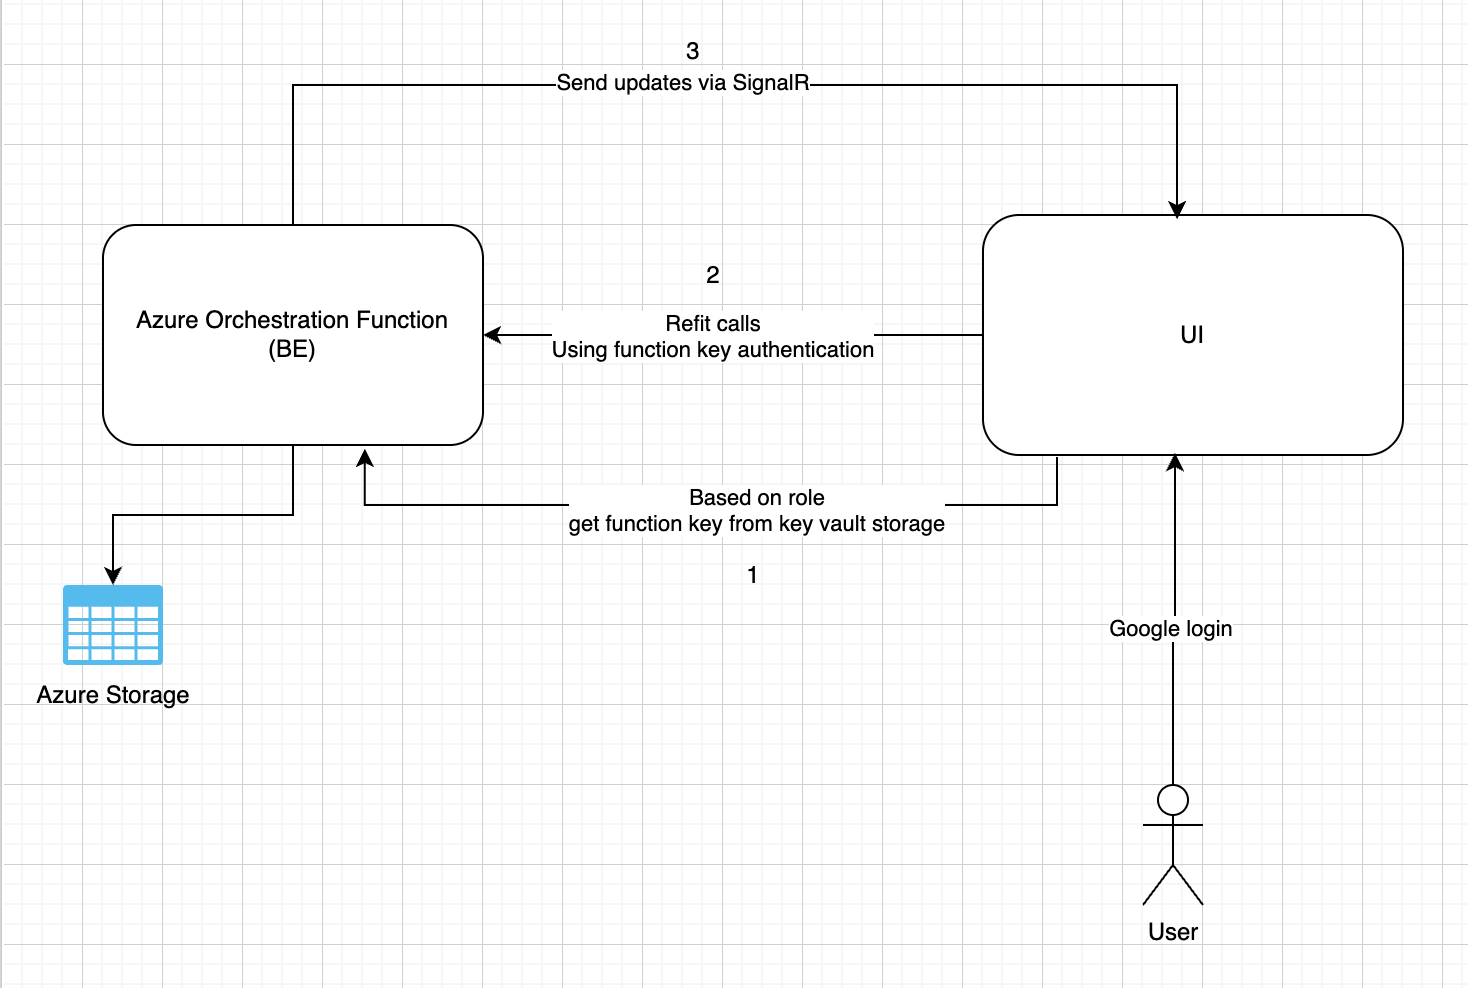
\includegraphics[width=14cm]{Assets/componentsComunication.png}
    \caption{Comunicarea dintre componentele proiectului}
    \label{fig:componentsComunication}
\end{figure}

\section{Arhitectura aplicației}
Aplicația dispunde de trei nivele:
\begin{itemize}
    \item stocare - unde se păstrează informațiile
    \item server-side - unde se prelucrează toate infomațiile
    \item client-side - unde se afisează toate informațiile către utilizatori
\end{itemize}

\subsection{Stocare}

Azure Table Storage este o bază de date NoSQL, ideală pentru scenarii în care se lucrează cu volume mari de date structurate,
dar fără relații complexe între entități. În cazul aplicației FastRide, fiecare entitate: utilizatori, curse, șoferi online și instanțele de orchestrare, este reprezentată ca o tabelă separată în Table Storage. Fiecare înregistrare (sau entitate) dintr-o tabelă este identificată în mod unic printr-o combinație de \textit{PartitionKey} și \textit{RowKey}, ceea ce asigură o distribuire eficientă și acces rapid la date.
\begin{figure}[H]
    \centering
    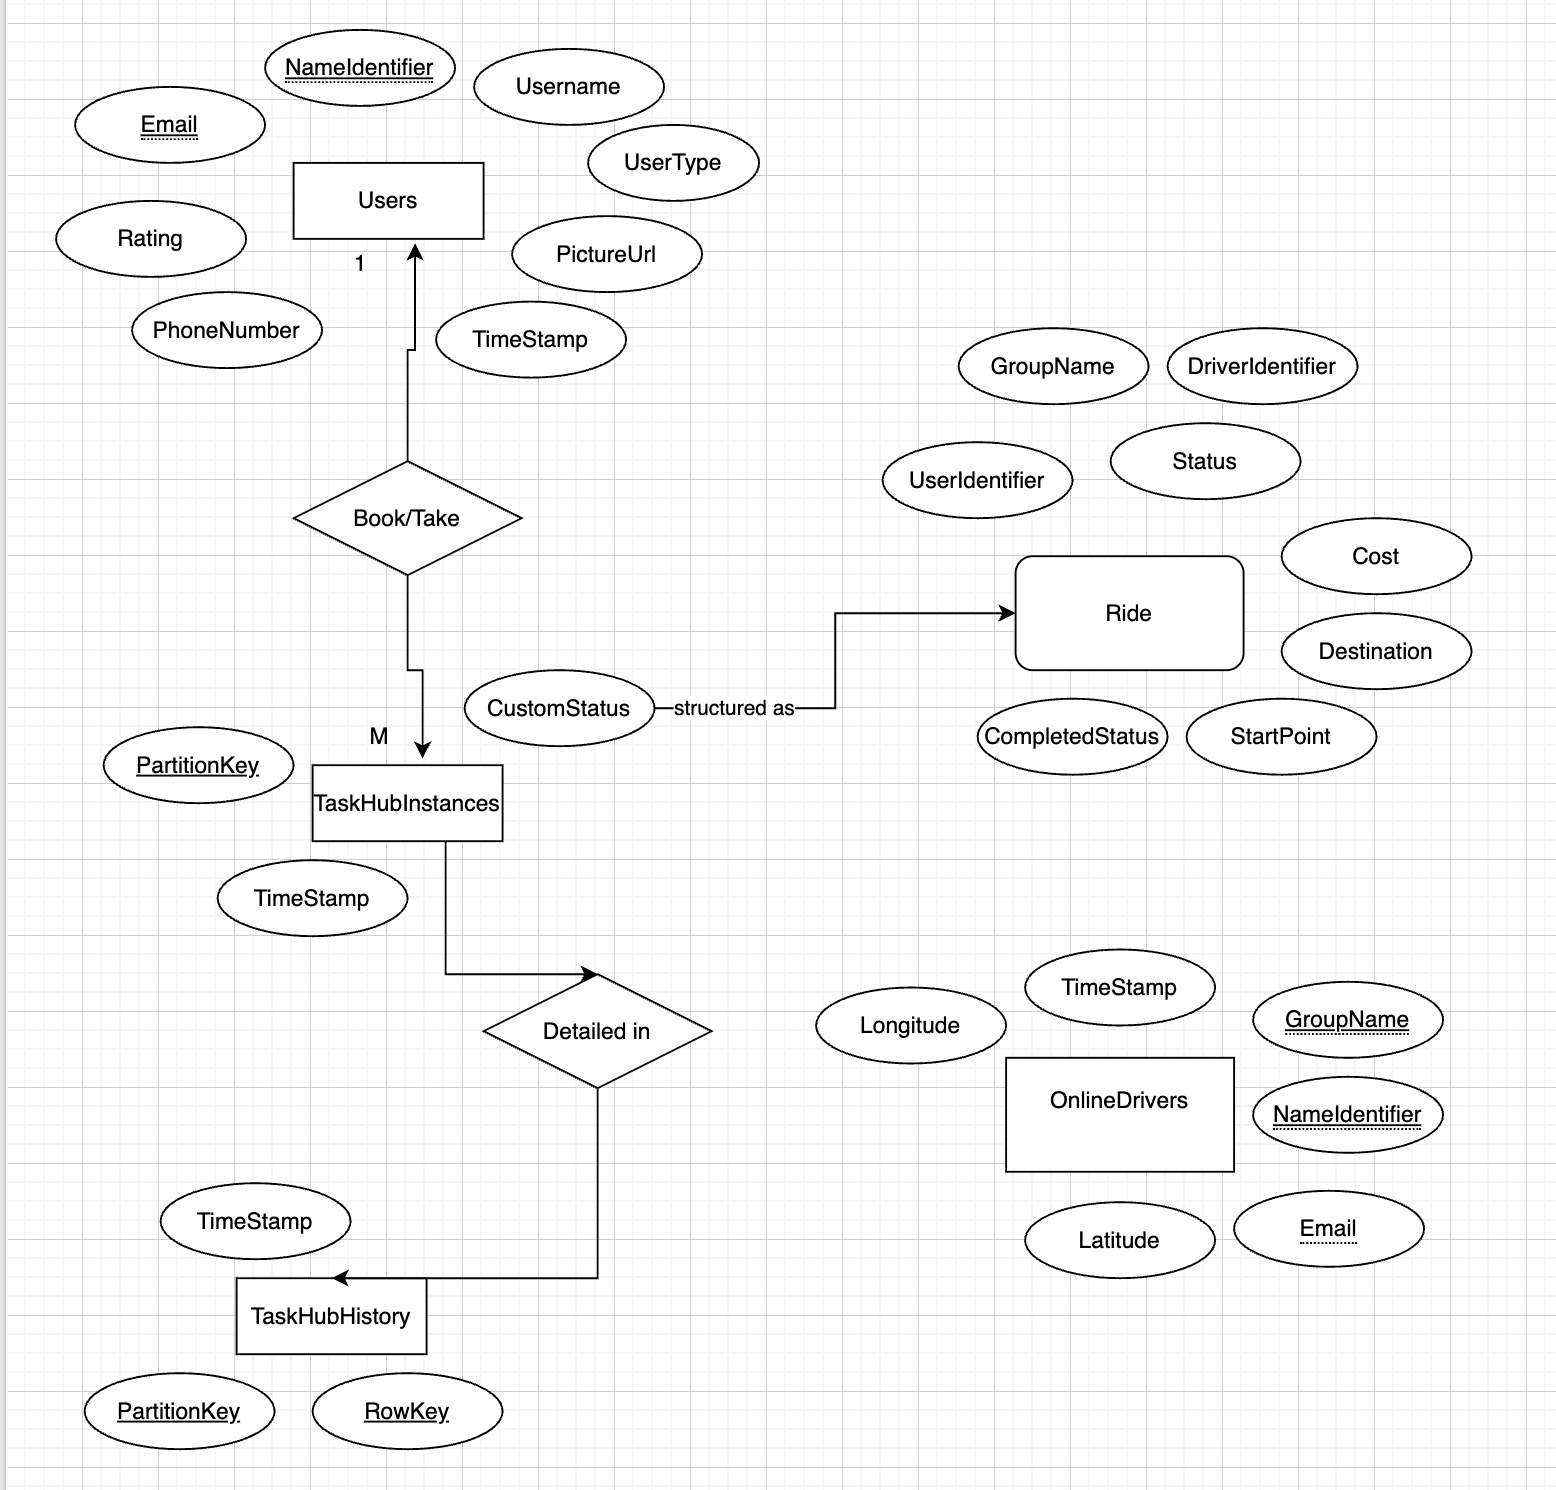
\includegraphics[width=14cm]{Assets/ER.png}
    \caption{Diagrama ER pentru baza de date.}
    \label{fig:ER}
\end{figure}

Aplicația FastRide conține trei entități, fiecare reflectând o componentă critică a funcționalității sistemului: utilizatorii, cursele și șoferii online.

Totul pornește de la entitatea \textit{Users}, care stochează informațiile de bază ale fiecărui utilizator autentificat prin Google.
Fiecare utilizator este identificat în mod unic prin \textit{NameIdentifier} și \textit{Email}, iar alături de acesta se păstrează date precum numele (\textit{Username}), tipul de utilizator (\textit{Driver}, \textit{User} sau \textit{Admin}), ratingul acumulat de-a lungul timpului, numărul de telefon și o eventuală poză de profil (\textit{PictureUrl}).

În momentul în care un utilizator rezervă sau preia o cursă, se creează o relație între acesta și instanțele de orchestrare.
Aici intervin tabelele \textit{TaskHubInstances} și \textit{TaskHubHistory}, care reflectă intern mecanismul
de orchestrare al Azure Durable Functions. Fiecare instanță a unei funcții durabile este stocată în \textit{TaskHubInstances}, iar starea
sa (\textit{CustomStatus}) este utilizată pentru a reflecta progresul unei curse (\textit{Ride}). În paralel, \textit{TaskHubHistory} păstrează detaliile cronologice ale
execuției, istoricul exact al fiecărei acțiuni legate de instanța respectivă. Ambele entități sunt identificate prin \textit{PartitionKey}, iar
în cazul istoricului, și prin \textit{RowKey}.

Starea unei curse este gestionată de modelul \textit{Ride}, care este corelat cu Users prin câmpul \textit{UserIdentifier}, indicând clientul
care a inițiat cererea. Dacă un șofer acceptă cursa, acesta este reprezentat prin \textit{DriverIdentifier}. Fiecare cursă este
caracterizată de un status:
\begin{itemize}
    \item \textit{NewRideAvailable} - status-ul inițial al cursei
    \item \textit{GoingToUser} - momentul în care șoferul acceptă cursa și navighează către client
    \item \textit{GoingToDestination} - atunci când șoferul merge spre destinație împreună cu pasagerul
    \item \textit{Finished} - cursa este finalizată cu success
    \item \textit{Cancelled} - cursa a fost anulată
    \item \textit{None} - state-ul inițial
\end{itemize}
Mereu după ce cursa se termina, aceasta se setează pe state-ul inițial.
Pentru a face vizibil în continuare statusul final al cursei, această memorează și un \textit{CompletedStatus} :
\begin{itemize}
    \item \textit{DriverNotFound} - nu s-a găsit niciun șofer pentru a finaliza cursa
    \item \textit{PaymentRefused} - clientul a refuzat plata (disponibilă doar cu cardul)
    \item \textit{Cancelled} - cursa este anulată din orice alte motive
    \item \textit{Completed} - cursa a fost terminată cu success
\end{itemize}
În infomațiile cursei se mai regăsesc și punctul de plecare (\textit{StartPoint}),
destinația (\textit{Destination}) și costul asociat. \textit{GroupName} este folosit pentru a lega această entitate de sesiunea real-time
corespunzătoare, utilă pentru actualizări prin SignalR, astfel încât, doar șoferii din același grup cu clientul ce a inițiat cursa pot interacționa.


Pe lângă aceste entități persistente, aplicația păstrează în mod temporar o listă cu șoferii activi prin tabela \textit{OnlineDrivers}.
Fiecare șofer online este identificat prin \textit{NameIdentifier} și asociat cu \textit{GroupName}, astfel încât să poată fi notificat
în timp real dacă există cereri în zona sa. Poziția sa curentă este păstrată prin coordonatele \textit{Latitude} și \textit{Longitude},
permițând localizarea sa pe hartă.

Azure Table Storage oferă performanță, scalabilitate și costuri reduse, iar modelul este suficient
de flexibil pentru a susține dezvoltări ulterioare, cum ar fi introducerea plăților reale, recenziilor textuale
sau programării curselor în avans.

\subsection{Server-side}

Backendul aplicației este construit folosind .NET și Azure Functions, oferind o arhitectură
serverless, scalabilă și eficientă pentru gestionarea întregii logici din spatele aplicației.
Totul pornește de la faptul că aplicația este construită într-un mod în care clientul
(Blazor WebAssembly) comunică prin HTTP și SignalR cu backendul, trimițând cereri sau
ascultând în timp real anumite evenimente.

Structura proiectului Server, este cuprinsă din mai multe layere: function triggers, orchestrations,
activities, services și repositories.

\textit{Function triggers} sunt de 3 tipuri: \textit{HttpTrigger}, \textit{TimeTrigger} și \textit{SignalRTrigger}.

HttpTriggers sunt folosite pentru comunicarea cu Client-side, și sunt requesturi de tipul Get/Post și Put.
\begin{figure}[H]
    \centering
    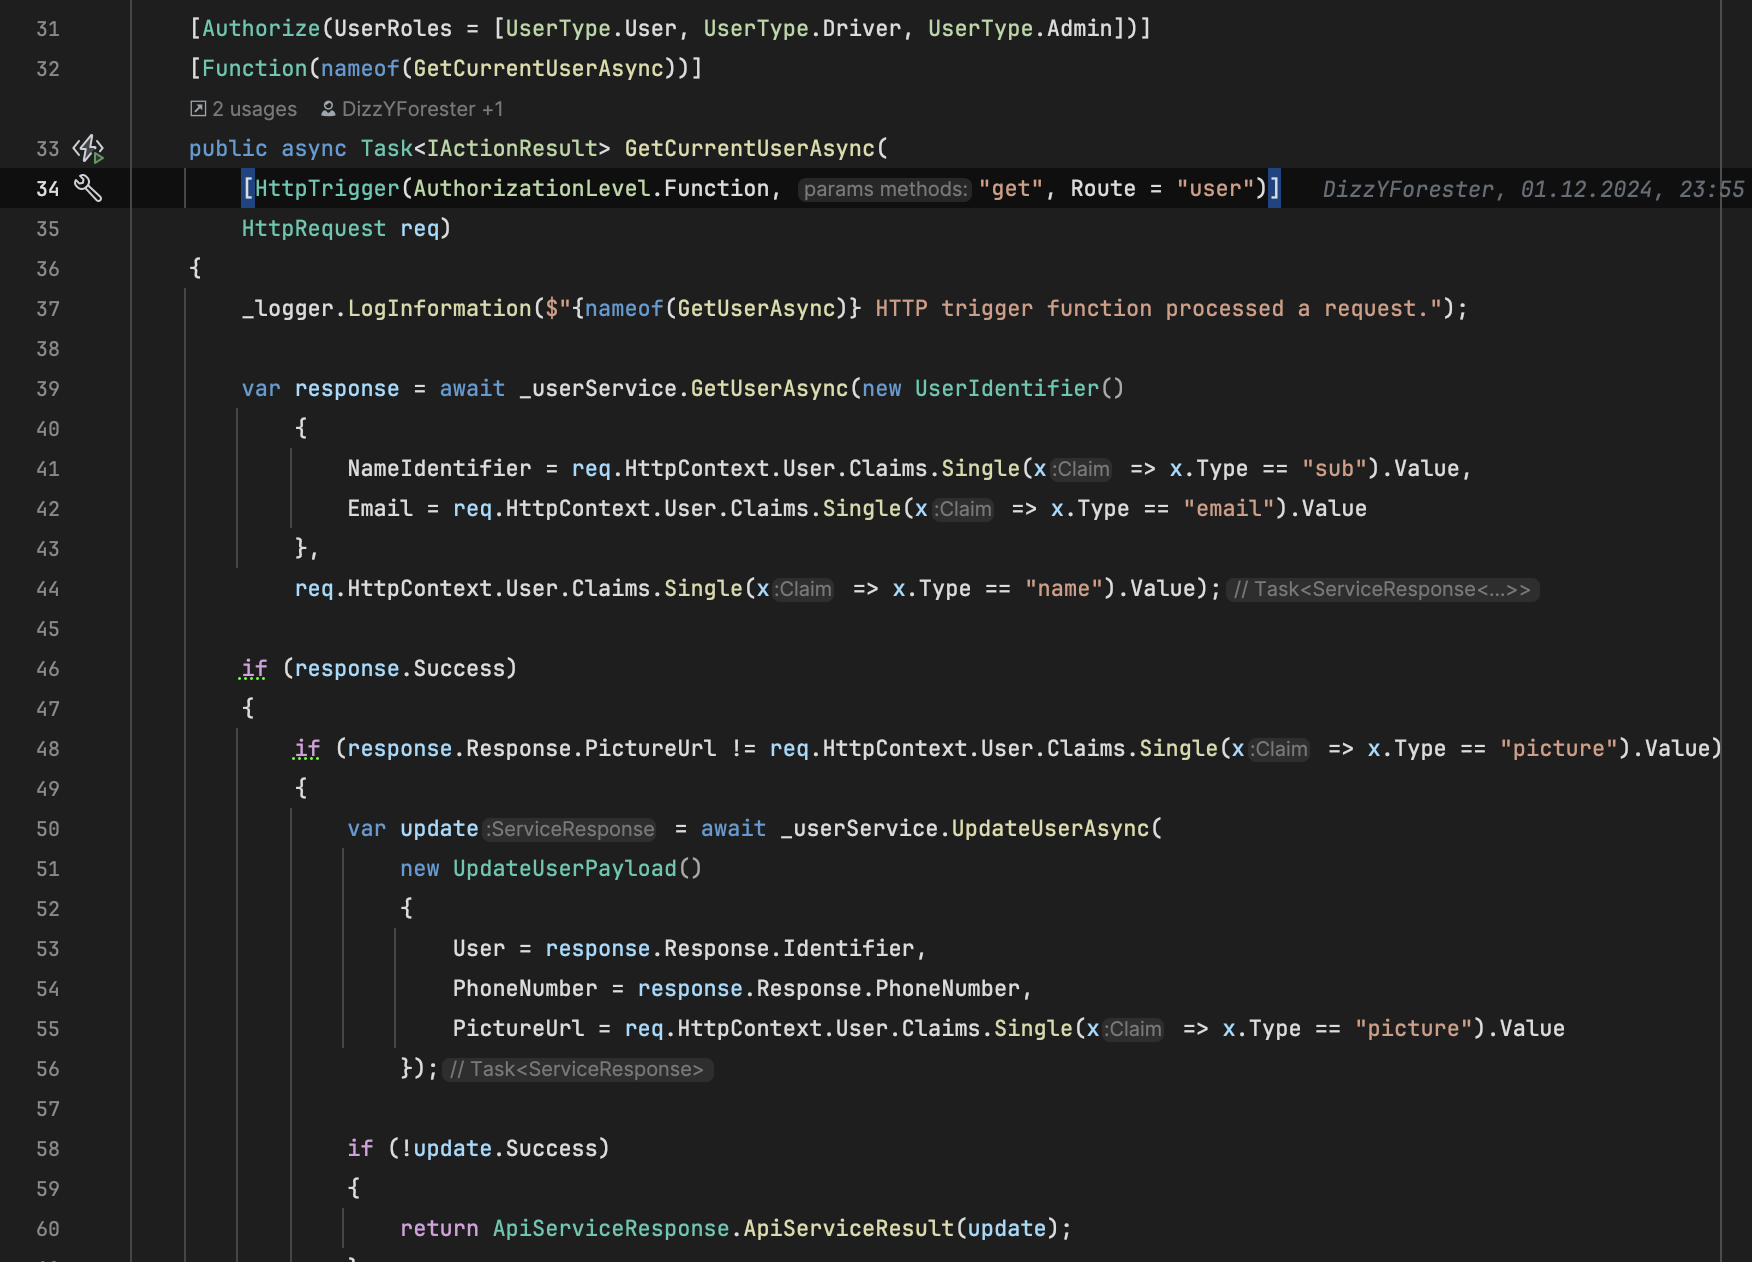
\includegraphics[width=14cm]{Assets/HttpTrigger.png}
    \caption{Exemplu de metodă GET pentru HttpTrigger function.}
    \label{fig:HttpTrigger}
\end{figure}

Aceste request-uri sunt autorizate prin Google token. Astfel s-a creat un atribut custom,
ce poate fi folosit doar pe methods, unde se pot defini o listă de \textit{roles} ce pot
accesa metoda respectivă.
Ca și request, body-ul este incapsulat în modelul \textit{HttpRequest} și poate fi deserializat
astfel:
\begin{figure}[H]
    \centering
    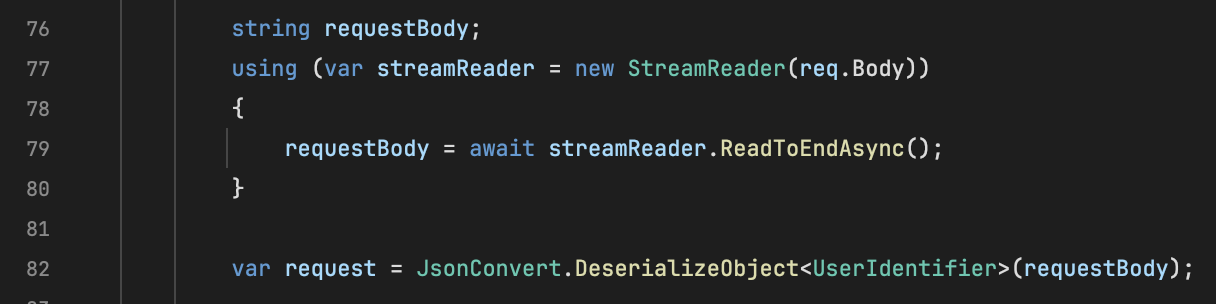
\includegraphics[width=14cm]{Assets/DeserializeRequest.png}
    \caption{Deserializarea unui request într-un tip concret (ex: \textit{UserIdentifier}).}
    \label{fig:DeserializeRequest}
\end{figure}

Ca și răspuns, toate Http functions întorc un \textit{IActionResult} ce este mapat dintr-un extension
pentru un \textit{ServiceResponse}. Acest model conține statusul request-ului, mesajul de eroare (dacă
există) și payload-ul response-ului. Toate service-urile conțin returnează un \textit{ServiceResponse}
care la fel, conține payload-ul, dacă este cu succes sau nu și mesajul de eroare împreună cu excepții.
Dacă există mesaj de eroare atunci rezultatul este un \textit{Bad Request (400)}, iar dacă există
excepție atunci se traduce ca \textit{Internal Server Error (500)}.

\begin{figure}[H]
    \centering
    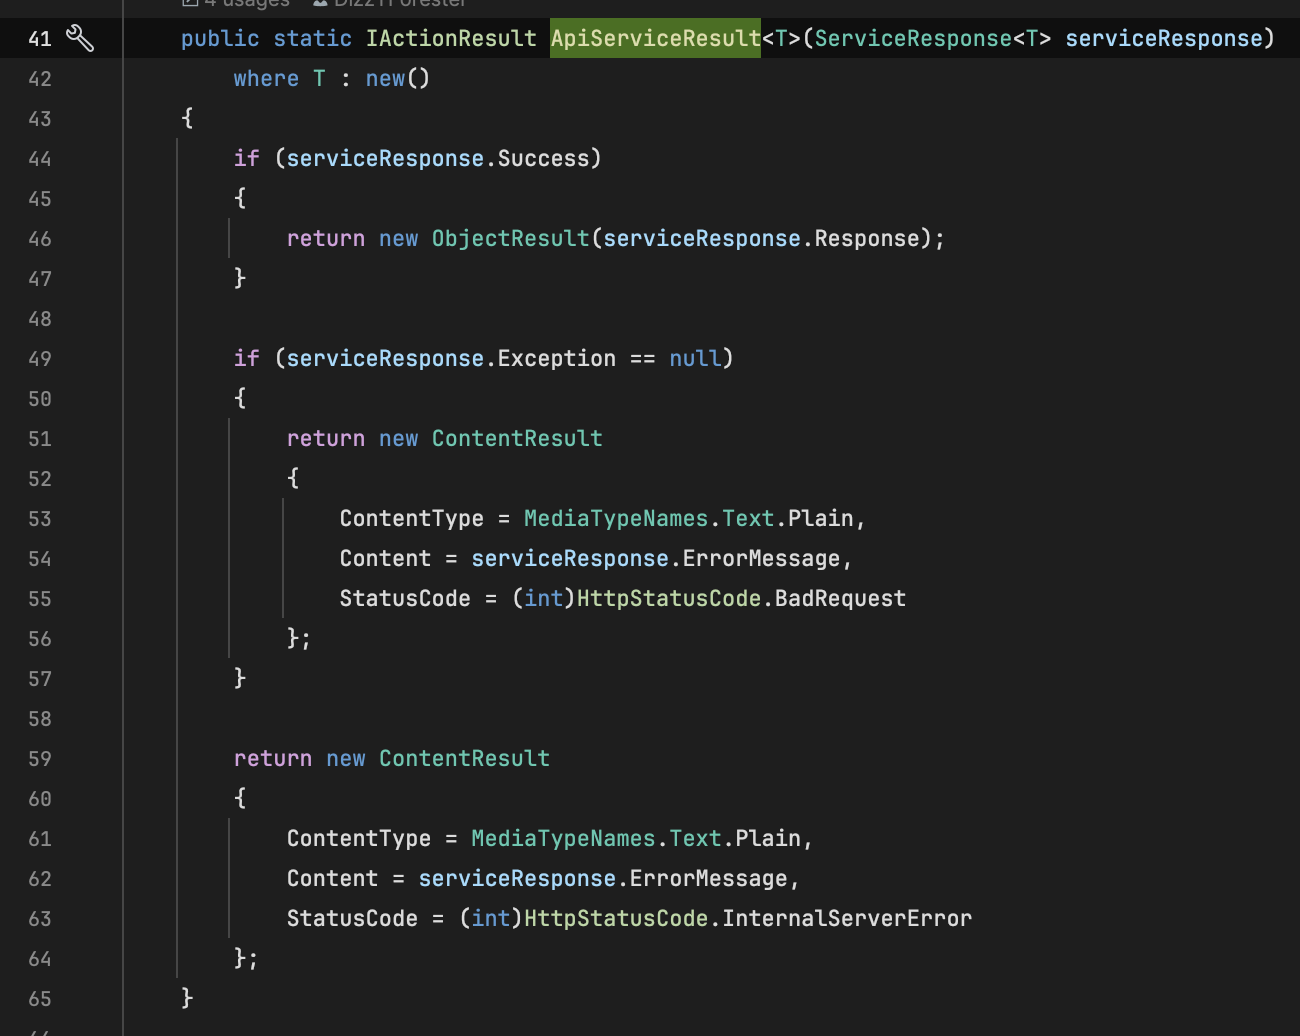
\includegraphics[width=14cm]{Assets/HttpResponse.png}
    \caption{Maparea unui \textit{ServiceResponse} la \textit{IActionResult}.}
    \label{fig:HttpResponse}
\end{figure}

Metodele HTTP disponibile pentru Client sunt:
\begin{itemize}
    \item \textit{GetCurrentUserAsync} pentru a lua informațiile despre user-ul de a inițiat requestul;
    \item \textit{GetUserAsync} pentru a lua informațiile despre un user;
    \item \textit{GetUsers}, disponibil doar pentru admini, pentru a vedea toți utilizatorii;
    \item \textit{UpdateUserAsync} pentru a actualiza un user;
    \item \textit{GetRidesByUserAsync} pentru a afișa cursele unui utilizator
\end{itemize}

Pentru a autoriza aceste endpoint-uri, în Azure Functions se pot înregistra \textit{middleware} pentru 
a verifica token-ul. Astfel \textit{AuthenticationMiddleware} și \textit{AuthorizationMiddleware} se ocupă de autentificarea 
și autorizarea API-ului, luând JWT token-ul din \textit{Authorization} header, și îl validează
folosind API-ul de la Google.

\begin{figure}[H]
    \centering
    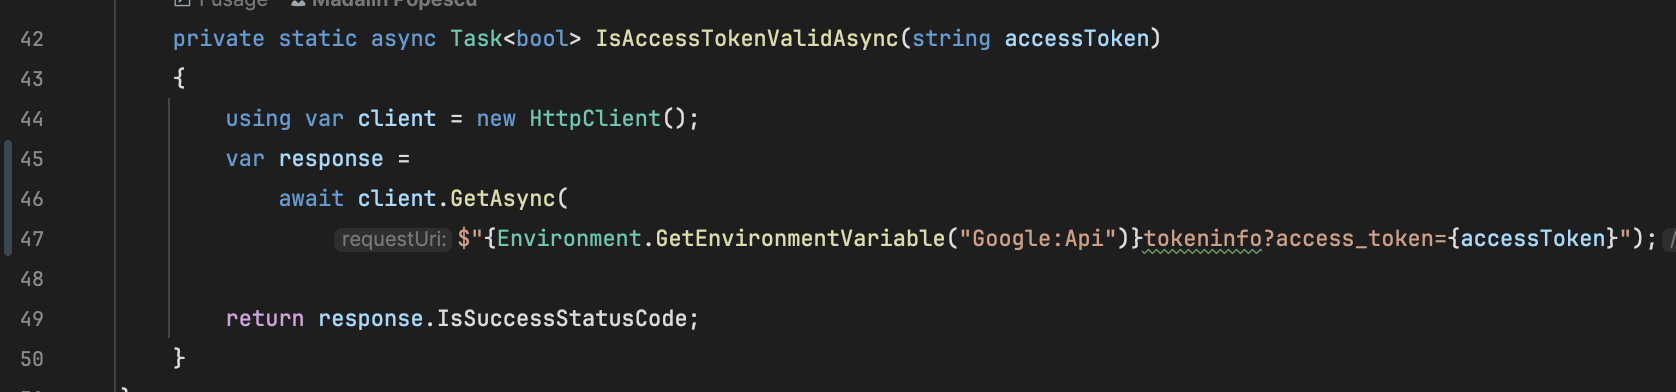
\includegraphics[width=14cm]{Assets/GoogleAuthorization.png}
    \caption{Verificare \textit{AccessToken} folosind Google API.}
    \label{fig:GoogleAuthorization}
\end{figure}

Pentru a face Google API conștient despre existența aplicației și token-ului pe care user-ul îl obține
prin autentificarea pe Client, în Google Console, se creează un \textit{Credential} pentru proiect.
Redirect URIs și request browser sunt reprezentate de Client URL (de acolo se apelează autentificarea).

\begin{figure}[H]
    \centering
    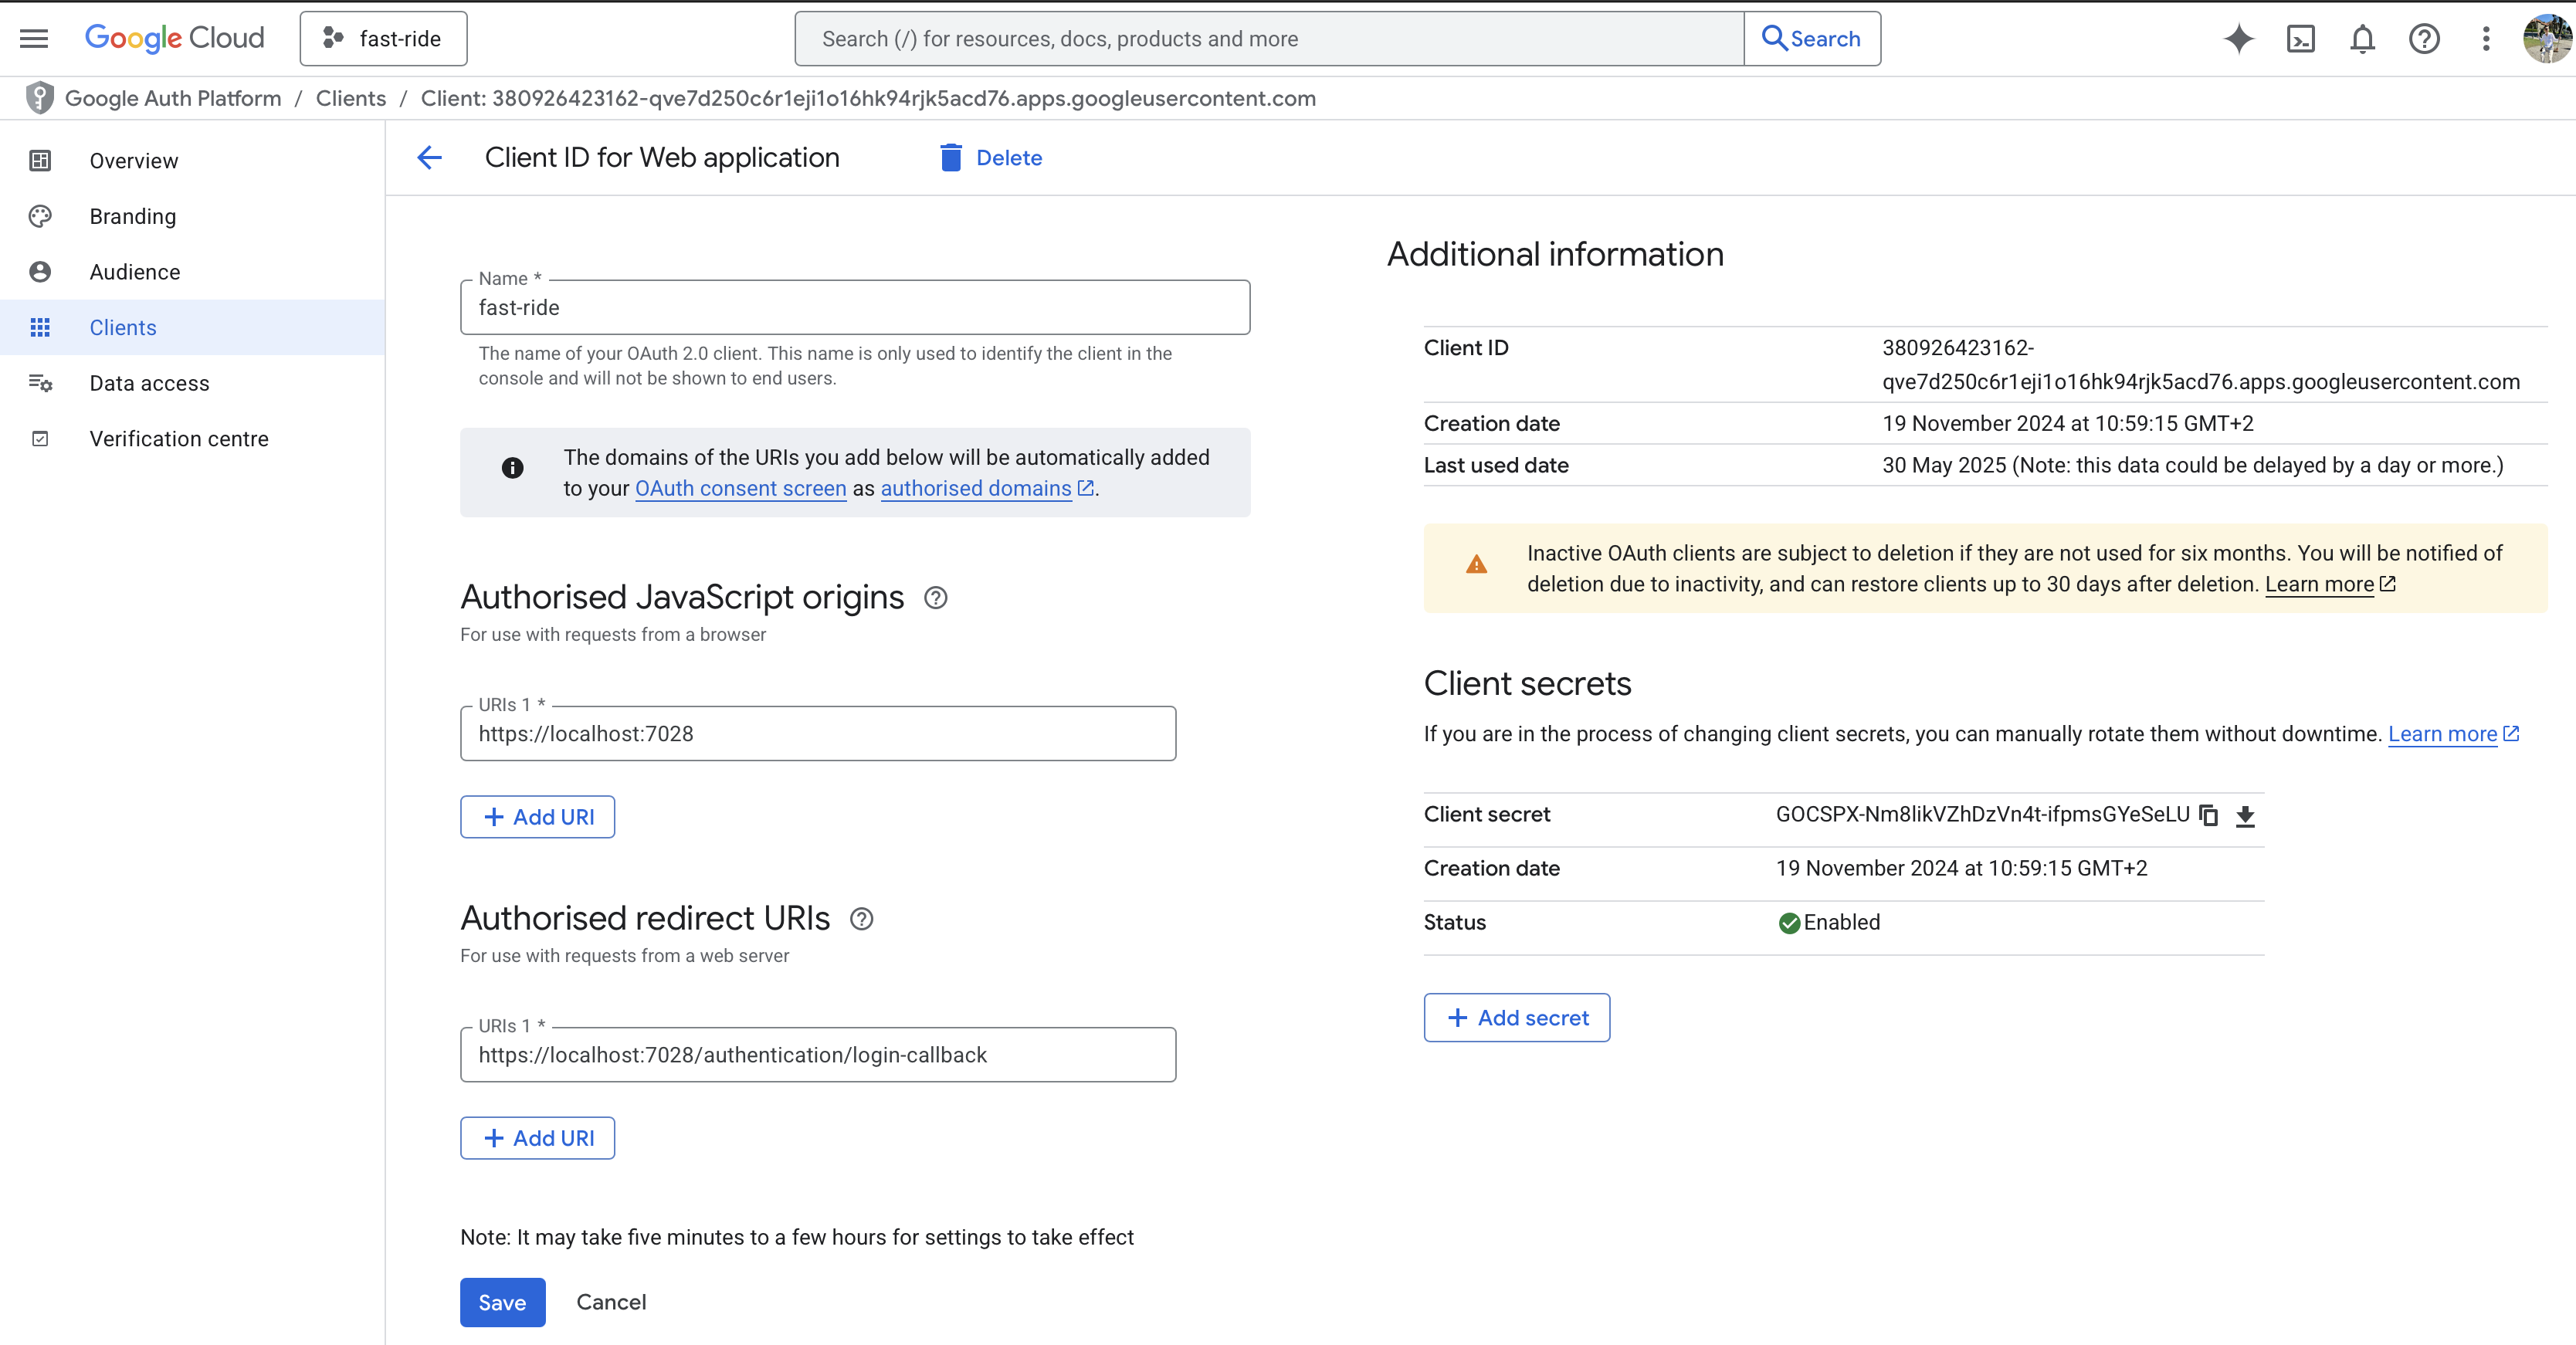
\includegraphics[width=14cm]{Assets/GoogleConfig.png}
    \caption{Configurația Google Credentials.}
    \label{fig:GoogleConfig}
\end{figure}

\textit{TimeTrigger} functions reprezintă funcțiile ce se auto-apelează la o perioadă de timp configurată.
FastRide folosește un acest tip de function pentru a interoga din 5 în 5 secunde tabelul generat
de Durable Orchestation în scopul de a găsi curse ce se află în progres și de a le notfica 
Client-ului prin SignalR.

\begin{figure}[H]
    \centering
    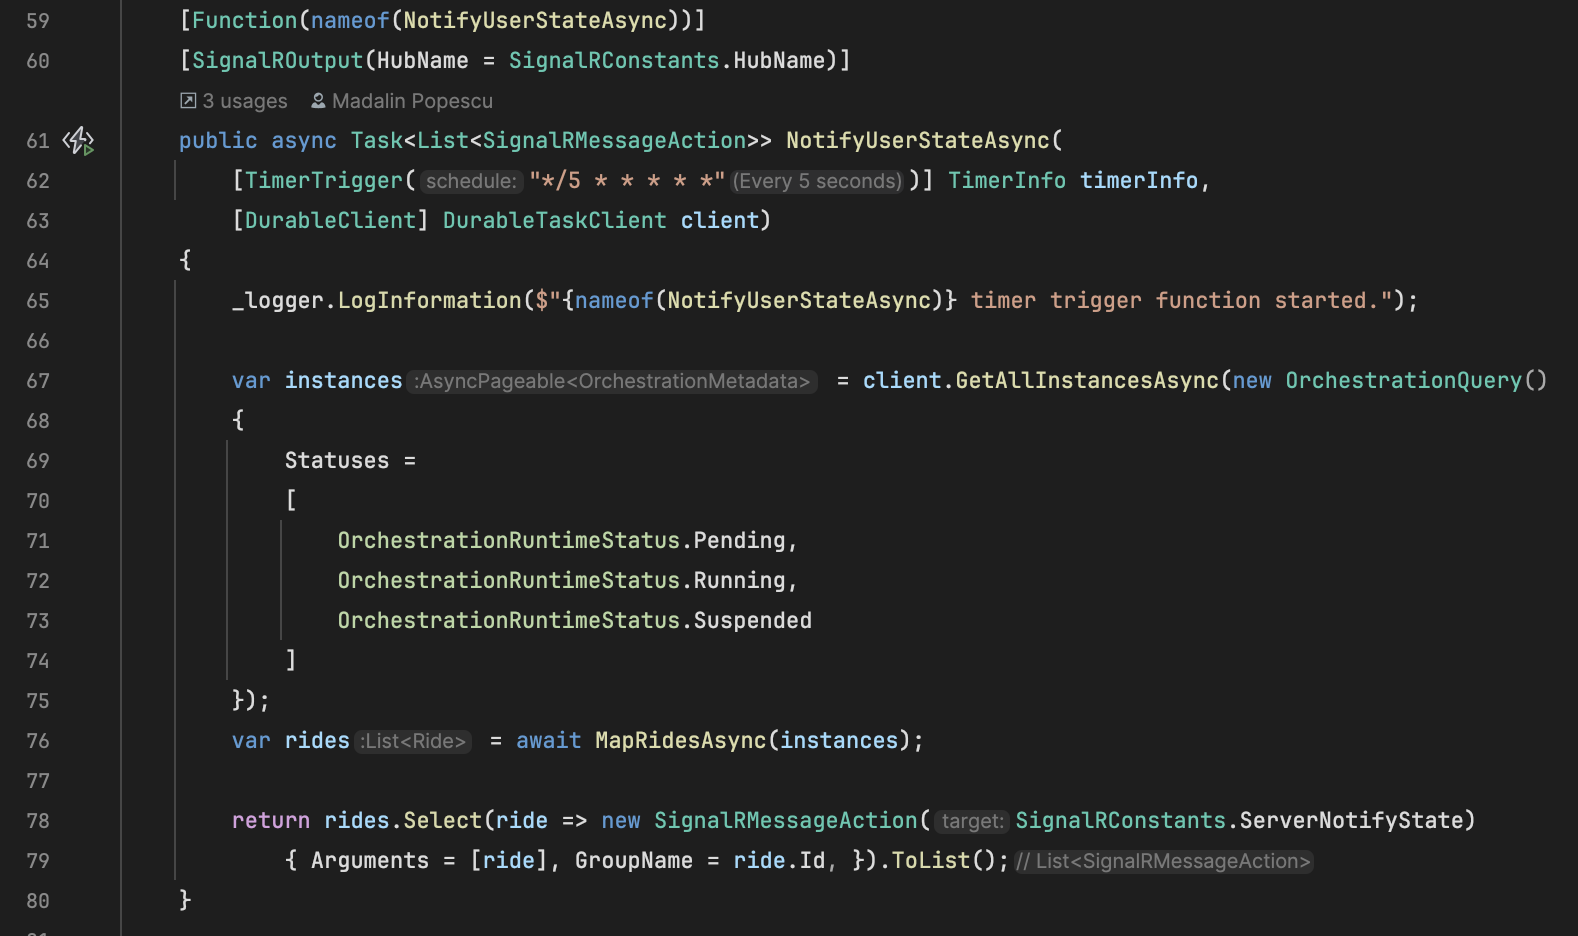
\includegraphics[width=14cm]{Assets/TimeTrigger.png}
    \caption{TimeTrigger function ce interoghează Durable tables și notifică utilizatorii despre curse lor ce sunt în desfășurare.}
    \label{fig:TimeTrigger}
\end{figure}
Aceasta caută orchestrările ce se află în \textit{Pending}, \textit{Running} sau \textit{Suspended},
citește proprietatea \textit{CustomStatus} unde se regăsesc informațiile complete ale cursei și 
le returnează pentru fiecare grup de utilizatori ce se află în parcursul unei curse (\textit{GroupName} este \textit{ride.Id}).

\textit{SignalRTrigger} sunt function-urile ce ascultă la un canal WebSocket pentru SignalR, dar sunt și capabile să returneze
un mesaj pe acest canal. Acestea sunt folosite pentru comunicarea în timp real cu Client-ul și au rolul de a notifica 
utilizatorii despre diferite acțiuni ce trebuie sa le facă (ex: plată, acceptare cursă, etc).
Acest tip de funcții folosesc un \textit{eventType} ca și identificator pentru a notifica utilizatorii ce sunt
conectați la canal. Utilizatorii pot fi grupați pe în grupuri pentru a trimite mesaje doar către un 
anumit grup, însă se pot trimite mesaje și direct către un utilizator specific.

FastRide folosește grupurile pentru a grupa utilizatorii per orașe, astfel cei din Craiova nu pot 
vedea și nu pot primi mesaje de la cei din București, spre exemplu. Grupurile se mai folosesc și 
pentru a identifica doi utilizatori ce se află într-o cursă, astfel în momentul în care o cursă se inițiază,
atât șoferul cât și clientul, părăsesc automat gurpul din care fac parte (o combinație dintre țară, județ și oraș) 
și se înscriu la grupul ce se formează din ID-ul cursei generat la creeare.

Pentru a se conecta la canalul de SignalR și pentru a se înscrie într-un grup sau pentru
a părăsi un grup, Client-ul trebui sa apeleze câteva metode care indică aceste \textit{actions}.

\begin{figure}[H]
    \centering
    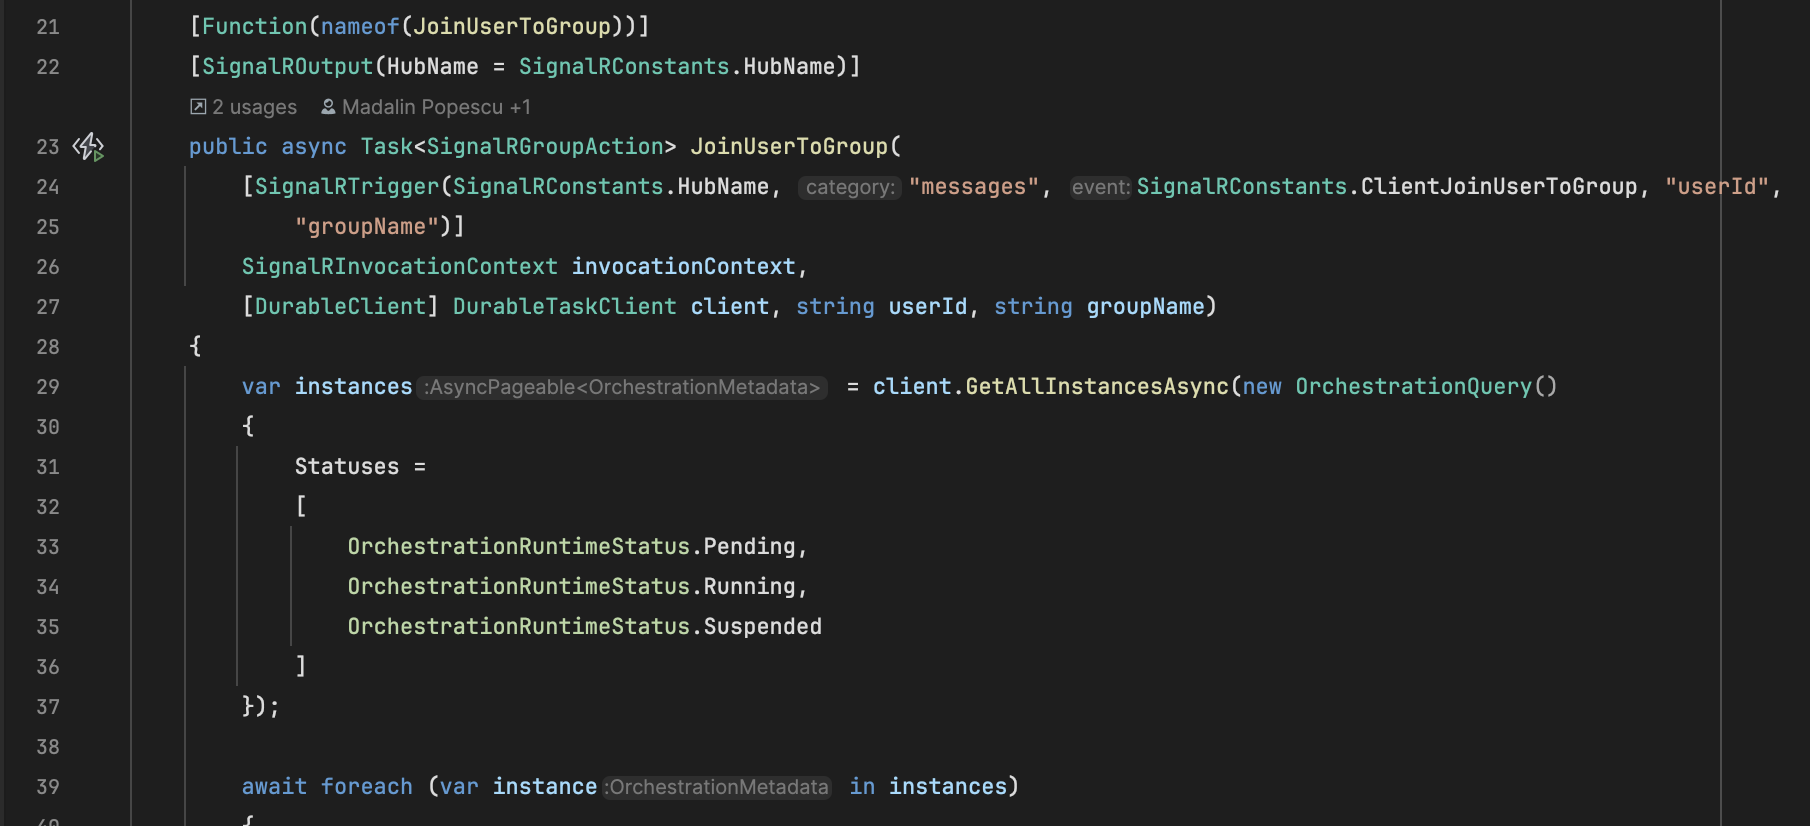
\includegraphics[width=14cm]{Assets/JoinUser.png}
    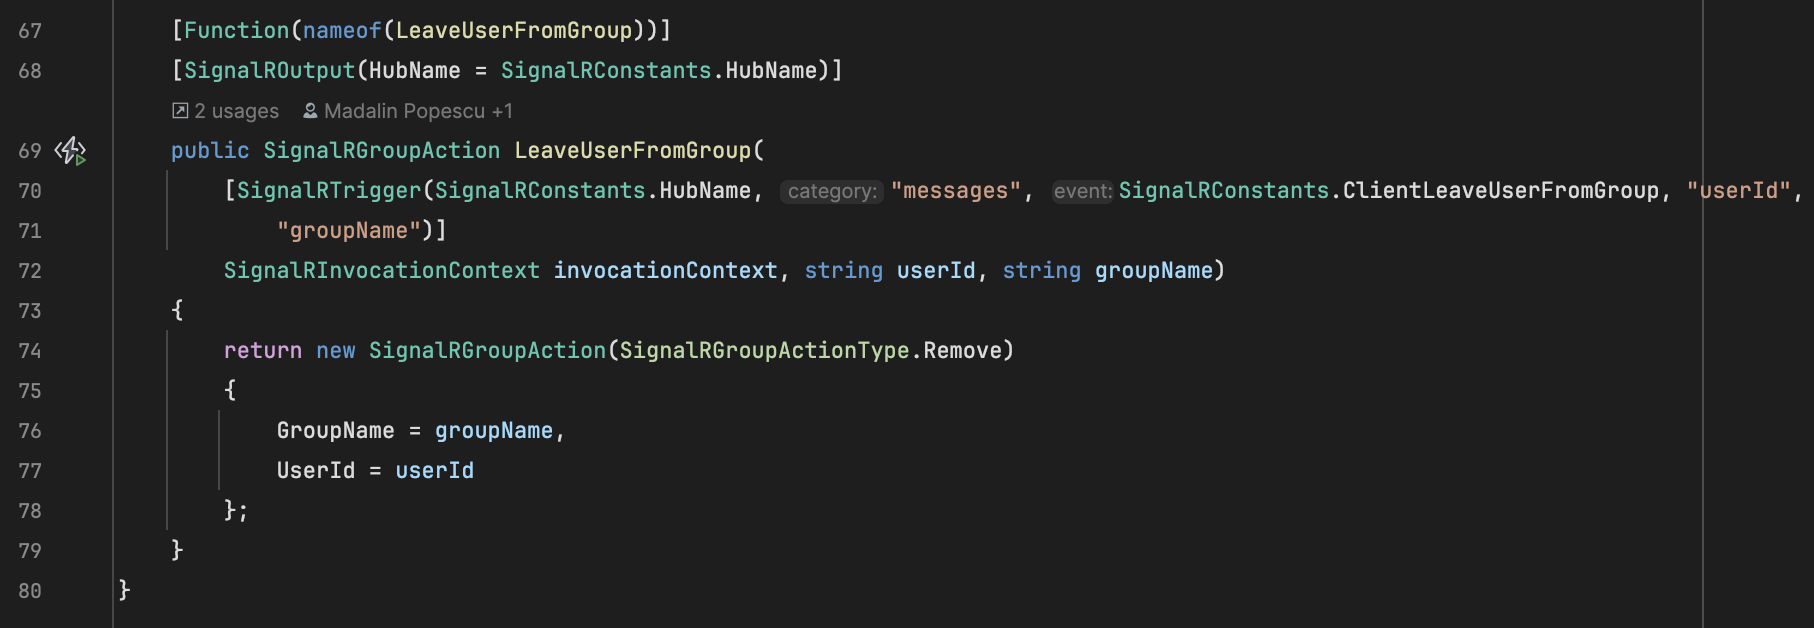
\includegraphics[width=14cm]{Assets/RemoveUser.png}
    \caption{Înscrierea și ștergerea unui utilizator din grup.}
    \label{fig:JoinRemoveUser}
\end{figure}

Pentru ca server-ul SignalR să înregistreze acțiunile aferente, Server-ul 
trebuie să returneze un \textit{SignalRGroupAction}. Pentru restul notificările 
se folosește \textit{SignalRMessageAction}.

Conectarea la SignalR de către utilizator și notificarea că a fost conectat sau 
deconectat cu succes se fac prin metodele de mai jos:
\begin{figure}[H]
    \centering
    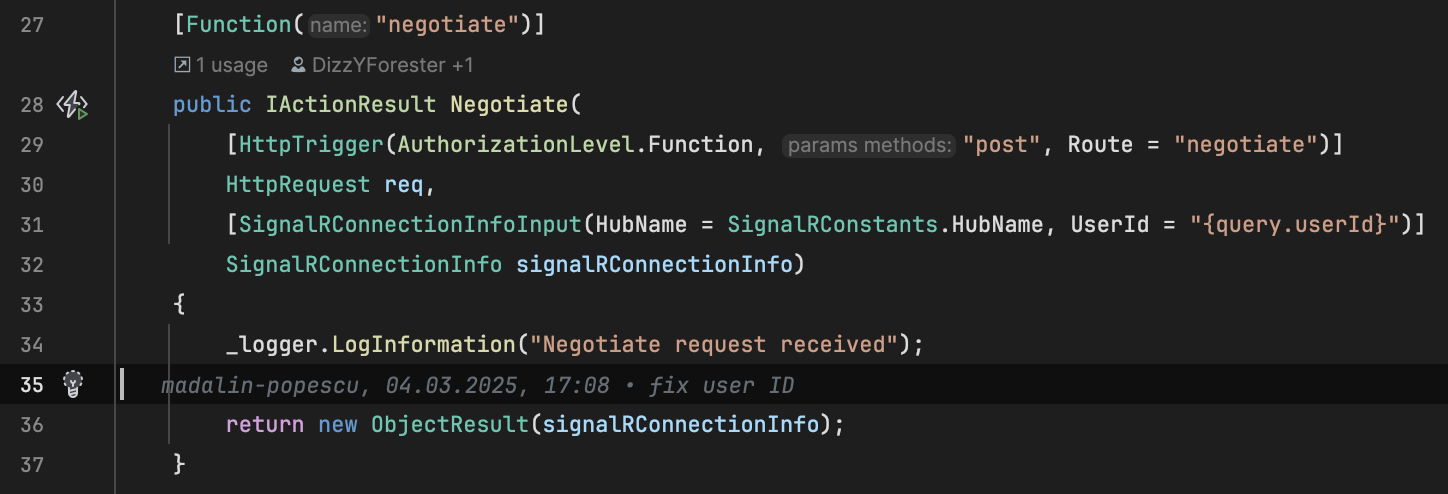
\includegraphics[width=14cm]{Assets/negotiate.png}
    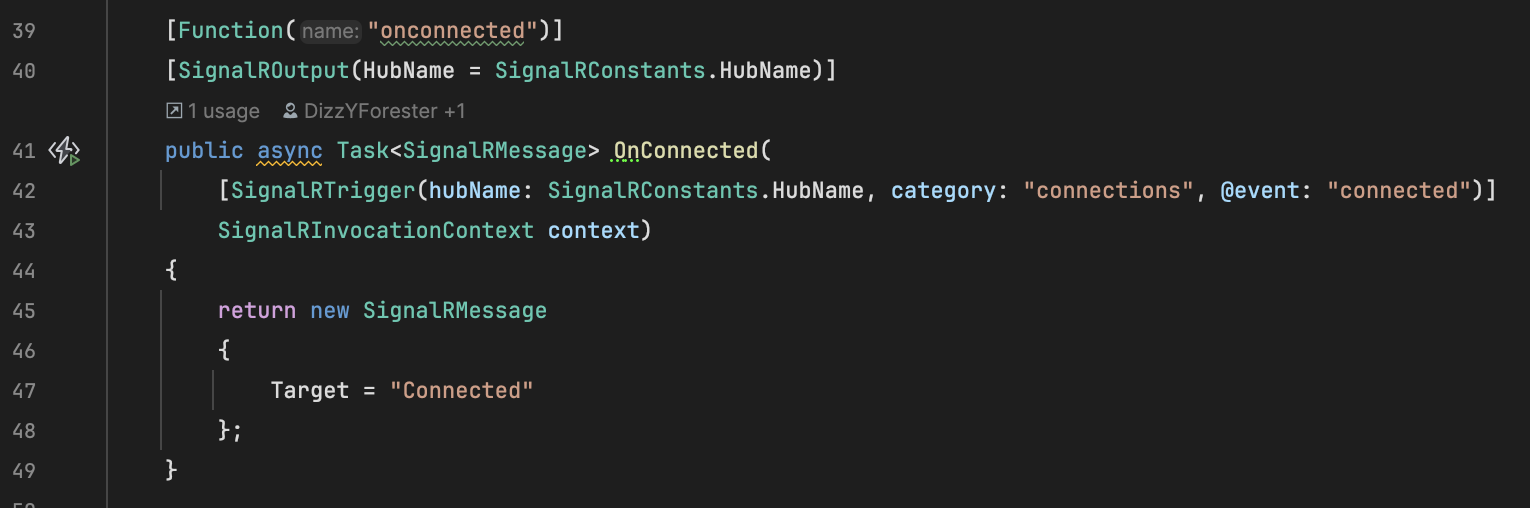
\includegraphics[width=14cm]{Assets/onconnected.png}
    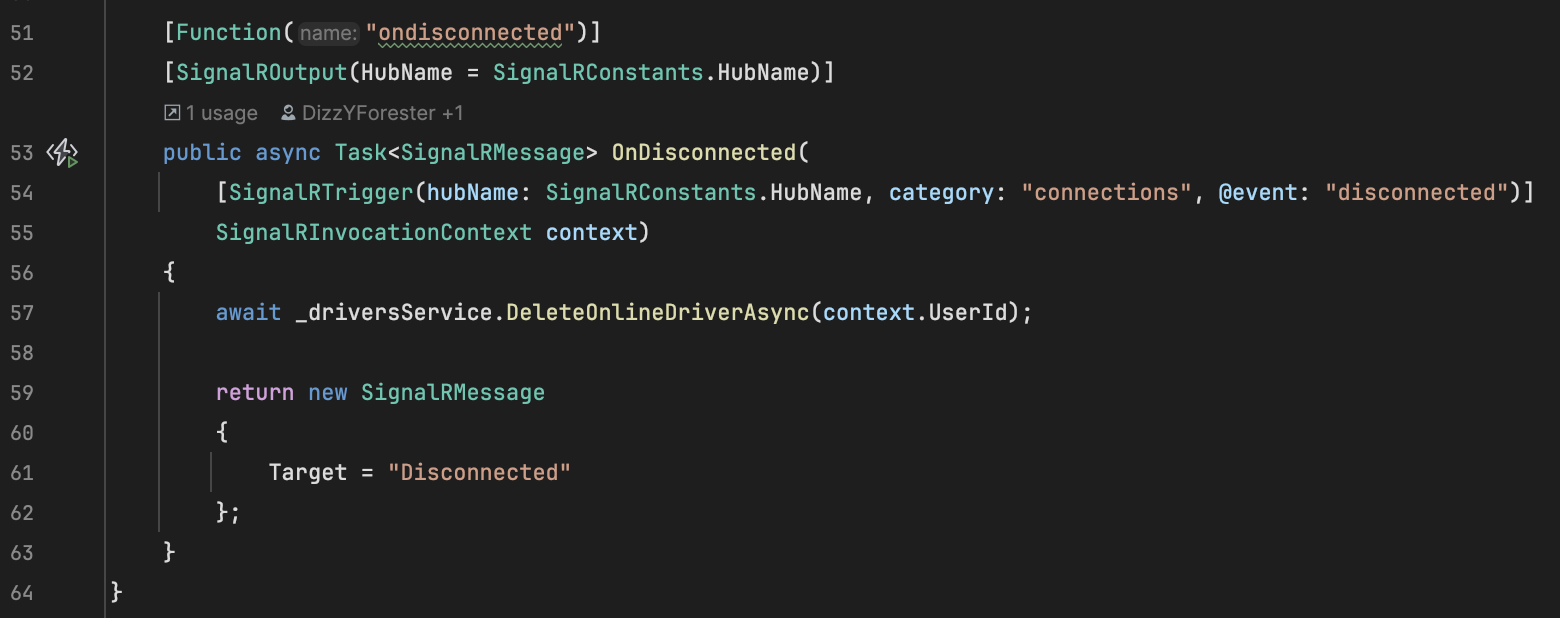
\includegraphics[width=14cm]{Assets/ondisconnected.png}
    \caption{Negotiate, conectarea și deconectarea unui utilizator de la conexiune SignalR.}
    \label{fig:negotiateConnectDisconnect}
\end{figure}
Astfel, în momentul în care un șofer este conectat sau deconectat, se poate actualiza
tabela \textit{OnlineDrivers}.

\textit{Orchestrations} sunt Azure Functions ce pot rula mai mult de 5 minute, ce își păstrează
state-ul în tabele, astfel încât indiferent de ce se întâmplă cu runtime-ul aplicației,
acestea își continuă execuția fără a relua tot procesul.

În proiect, există o singură funcție de acest gen, ce se ocupă cu flow management-ul unei curse.
Astfel, ea primește ca și input, un request ce conține \textit{User} (clientul), locul de unde se inițiază
cursa și destinația dorită. La fiecare pas, aceste infomații se actualizează și 
se salvează în coloana specială a Durable Orchestrations, \textit{CustomStatus}, totodată, modificând și status-ul
cursei.

\begin{figure}[H]
    \centering
    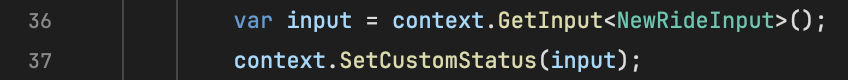
\includegraphics[width=14cm]{Assets/saveCustomStatus.png}
    \caption{Salvarea în \textit{CustomStatus} a request-ului inițial.}
    \label{fig:saveCustomStatus}
\end{figure}

Mai departe, aplicația calculează prețul cursei și trimite către utilizator un request de confirmare a cursei.
Pentru a aștepta răspuns, Durable Orchestrations folosesc evenimente pe care le așteaptă:
\begin{figure}[H]
    \centering
    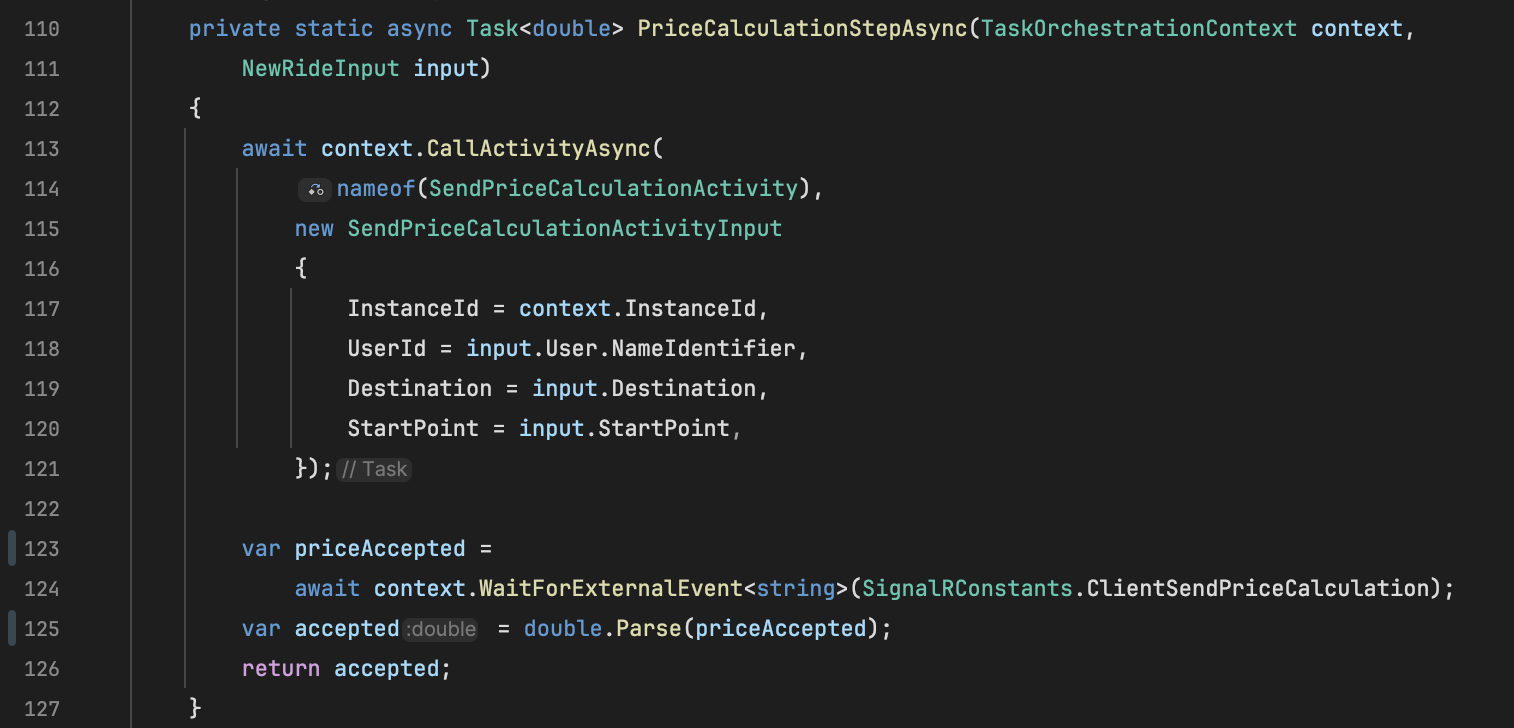
\includegraphics[width=14cm]{Assets/waitForEvent.png}
    \caption{Trimiterea confimării către utilizator și așteptarea răspunsului.}
    \label{fig:waitForEvent}
\end{figure}
Pentru a calcula prețul se folosește următoarea formulă (distanța dintre 2 puncte în spațiu, estimarea timpului de
parcurgere cu un timp comun și prețul configurat pentru fiecare kilometru și minut adunat cu o sumă inițială):
\begin{figure}[H]
    \centering
    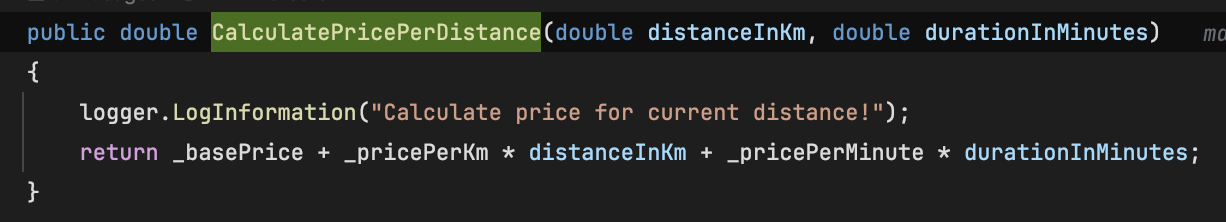
\includegraphics[width=14cm]{Assets/calculatePrice.png}
    \caption{Calcularea prețului cursei.}
    \label{fig:calculatePrice}
\end{figure}
Dacă s-a acceptat, urmează să se inițieze plata, astfel, Server-ul se ocupă cu creearea
unui \textit{PaymentIntent} ce se poate folosi pentru a se realiza plata cu succes. Fără acestă intenționare,
Stripe nu știe să autentifice request-ul de plată.
\begin{figure}[H]
    \centering
    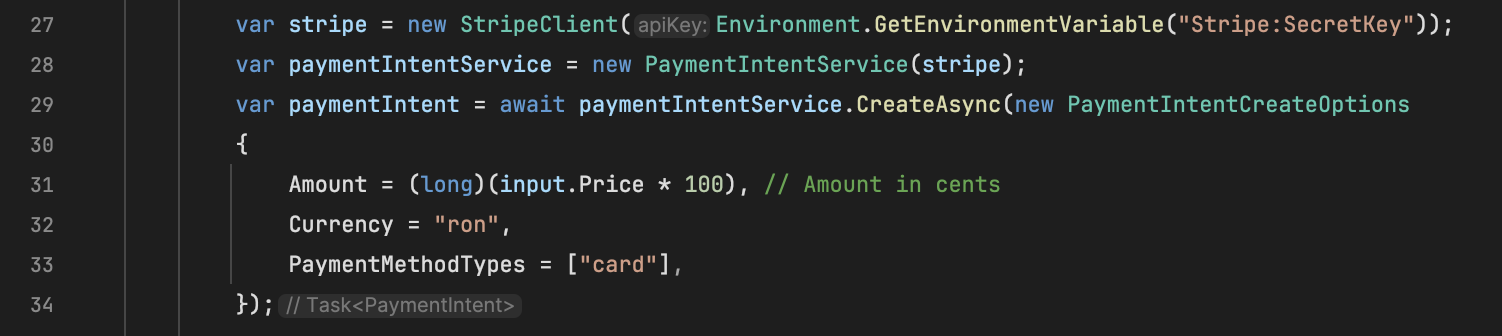
\includegraphics[width=14cm]{Assets/intent.png}
    \caption{Crearea \textit{PaymentIntent}-utului prin Stripe.}
    \label{fig:intent}
\end{figure}
Mai departe, după ce plata s-a procesat cu success, începe să se caute un șofer pentru cursă.
Algoritmul de căutare se folosește de tabelul \textit{OnlineDrivers} pentru a identifica poziția
fiecărui șofer și a îi calcula distanța de la client la acesta. Șoferii se iau în ordine până se găsește 
unul sau niciunul. Dacă șoferul nu acceptă cursa în timp de 35 secunde, se consideră ca și respinsă.
Pentru a face acest lucru posbil, se creează o listă de \textit{Task}, returnată de \textit{WaitForExternalEvent},
și așteaptă ca cel puțin unul din task-uri să se completeze. În funcție de task-ul completat, se alege
acțiunea de a merge mai departe sau de a căuta alt șofer.

\begin{figure}[H]
    \centering
    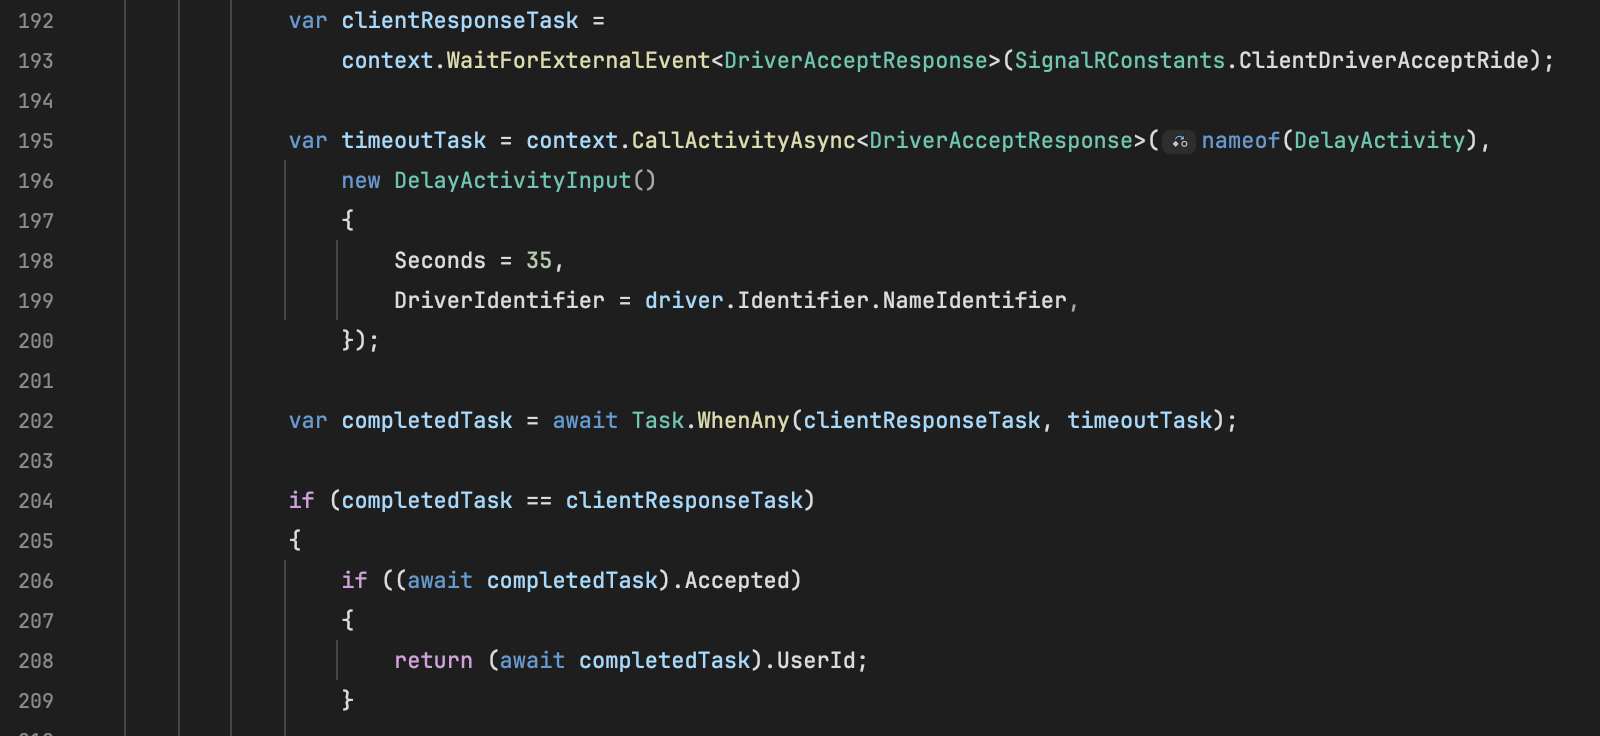
\includegraphics[width=14cm]{Assets/WaitForDriver.png}
    \caption{Așteptarea răspunsului de la șofer și cronometrarea timpului de acceptare.}
    \label{fig:WaitForDriver}
\end{figure}

La orice pas, dacă utilizatorul anulează fie confirmarea, fie plata, fie nu se găsește un șofer, cursa intră într-un status
terminal, setând proprietatea \textit{CompletedStatus} cu un status aferent acțiunii.
\begin{figure}[H]
    \centering
    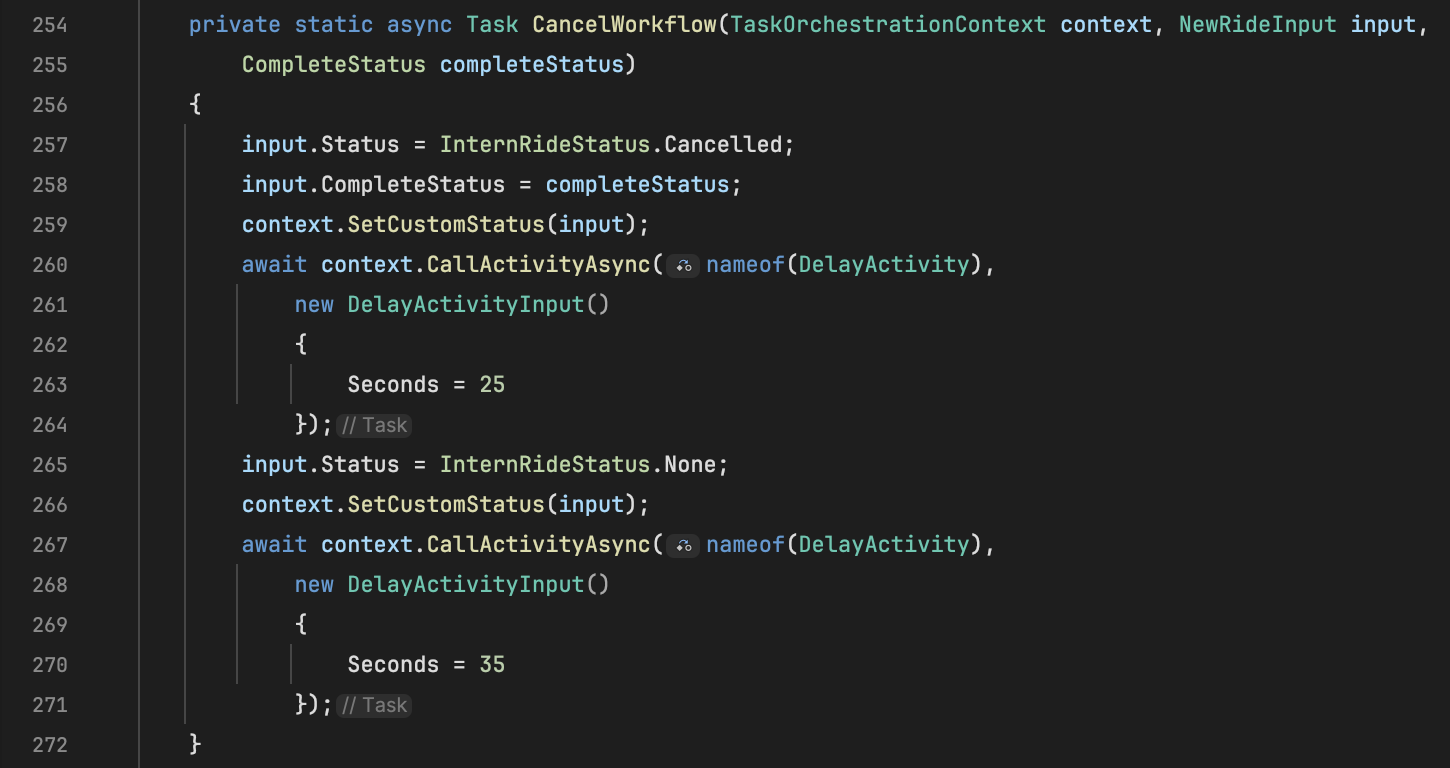
\includegraphics[width=14cm]{Assets/cancelFlow.png}
    \caption{Anularea cursei dacă plata nu s-a procesat, a fost intenționat anulată sau nu s-a găsit un șofer.}
    \label{fig:cancelFlow}
\end{figure}
Delay-urile au rolul de a face posibilă așteptarea ca și utilizatorul să primească aceste informații, altfel totul ar fi instant,
iar utlizatorul nu ar vedea niciun feedback.

Funcțiile durabile de orchestrare trebuie să fie deterministice, astfel încât dacă aplicația repornește
sau un proces de resetare intervine, codul să rezulte același rezultat. Pnetru asta, trebuie evitate în contextul
orchestration-ului să se genereze valori random sau să se apeleze service-uri. Totuși, este nevoie să se apeleze service-uri precum
calcularea pretului cursei sau căutarea unui șofer. Pnetru a face posibil acest lucru, intervin activtățile.

\textit{Activity functions} sunt funcții ce au rol de a menține pasul la care orchestration-ul rulează.
Pentru fiecare acțiune necesară în orchestration, există o activitate, astfel:
\begin{itemize}
    \item \textit{CancelRideActivity} - folosită pentru trimite cererea de anulare a cursei către toți participanții;
    \item \textit{DelayActivity} - folosită pentru a suspenda orchestration-ul pentru \textit{n} secunde;
    \item \textit{FindDriverActivity} - activitatea ce caută un șofer pentru cursa trimisă. Totodată, se trimite și lista de șoferi ce au fost excluși, datorită respingeri cererii;
    \item \textit{NotifyDriverTimeoutActivity} - notifică șoferul că perioada de acceptare a cursei a expirat;
    \item \textit{SendPaymentIntentActivity} - creează \textit{PaymentIntent}-ul și îl trimite către client;
    \item \textit{SendPriceCalculationActivity} - calculează prețul cursei și îl notifică pe client despre acesta;
    \item \textit{SendRatingRequestActivity} - la finalul cursei, clienții trebuie să ofere un notă șoferului, această activitate ocupându-se de această sarcină;
    \item \textit{SendRideToDriverActivity} - notifică șoferul despre cursă, acesta fiind nevoit să decidă dacă acceptă cursa sau nu.
\end{itemize}

\begin{figure}[H]
    \centering
    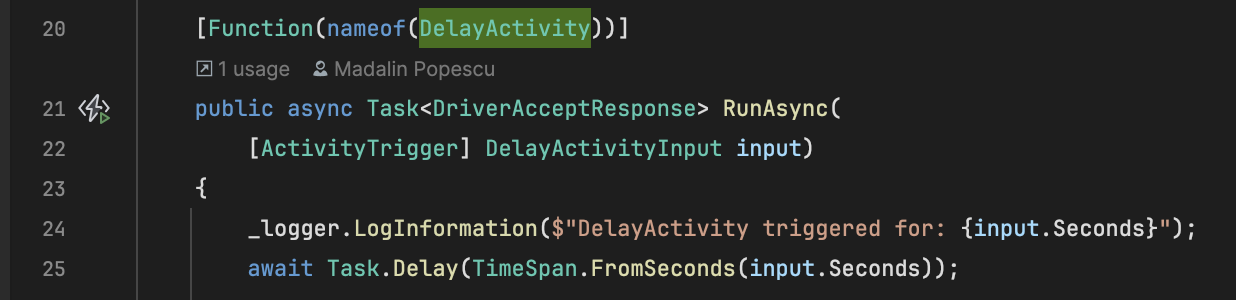
\includegraphics[width=14cm]{Assets/activities.png}
    \caption{Declararea activității ce pune orchestration-ul să aștepte \textit{n} secunde.}
    \label{fig:activities}
\end{figure}

Pentru a structura logica, separat de activități, se folosesc servicii. \textit{Services} sunt instanțe de clase înregistrate în
contextul aplicației pentru a putea fi injectate mai târziu, și folosite ca să execută diferită logică.
Spre exemplu, calcularea distanței dintre două puncte este o metodă dintr-un service înregistrat \textit{Scoped} (se generează o instanță nouă
la fiecare request inițiat). Alte servicii ce se regăsesc în proiect sunt pentru calcularea prețului, pentru 
a găsi șoferi apropiați de un client și de a intermedia operațiile \textit{CRUD} (Create Read Update Delete) pentru utilizatori și curse.
Toate serviciile folosesc o structură comună de returnare a datelor, răspunsul fiind încapsulat într-un \textit{ServiceResponse}
ce conține payload-ul, un mesaj de eroare sau o excepție, dacă există și dacă totul s-a executat cu succes sau nu. Acest tip de răspuns
ajută la handle-uirea răspunsului și încapsularea lui într-un \textit{ApiResponse}.

Configurarea proiectului se face prin \textit{Environment Variables}, local, definindu-se prin
\textit{local.settings.json}. Această configurație este alcătuită din:
\begin{itemize}
    \item Google Credentials - pentru a reuși validarea token-ului de acces ce vine pe request;
    \item Distance Configuration - ce conțin prețurile pentru un kilometru, un minut, prețul inițial și viteza medie de calcul pentru distanță;
    \item Stripe Secret Key - folosit pentru generarea inteționării de plată;
    \item Storage Connection String - conexiunea la Azure Storage.
    \item SignalR Connection String - conexiunea la server-ul SignalR
\end{itemize}

Microsoft, loghează fiecare activitate ce se execută, iar în caz de deployment pe o infrastructură ce permite logging (spre exemplu Azure),
este necesar să se specifice ce anume să se logheze pentru a nu se ajunge la costuri mari
\begin{figure}[H]
    \centering
    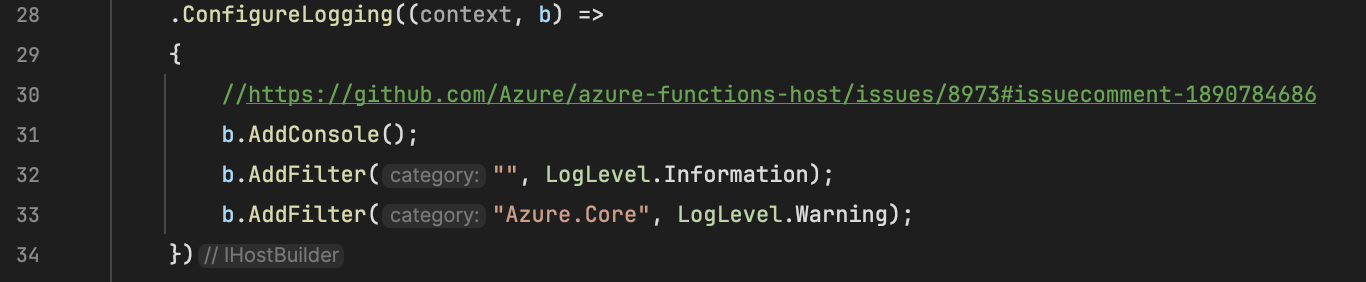
\includegraphics[width=14cm]{Assets/configLogging.png}
    \caption{Filtrarea log-urilor din Azure.}
    \label{fig:configLogging}
\end{figure}

\subsection{Client-side}

Client-side-ul se ocupă cu afișarea informațiilor procesate pe Server. La bază, stă
Blazor WASM, ce funcționează fără a avea nevoie de o componentă de server sau să instanțieze
două componente de comunicare. Toate asset-urile se descarcă în browserul utilizatorului și poate funcționa fără conexiune la internet.

Folderul \textit{wwwroot} este rădăcina conținutului static al aplicației Blazor WebAssembly. 
Tot ce se află în acest folder (sau în subfolderele lui) este expus publicului și servit direct browserului, fără procesare pe server.
Aici se regăsesc configurația proiectului pentru debugging, stilurile CSS, logica JavaScript, dar și datele mock pentru debugging.

\begin{figure}[H]
    \centering
    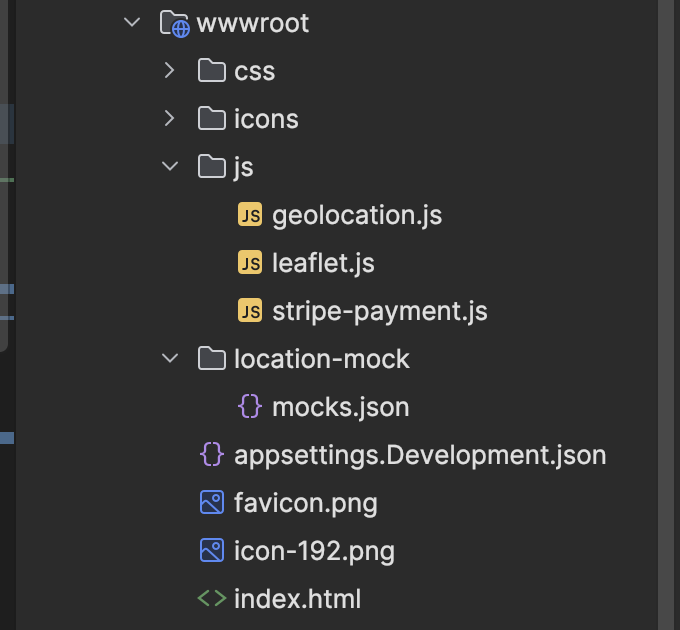
\includegraphics[width=10cm]{Assets/wwwroot.png}
    \caption{Conținutul folderului \textit{wwwwroot}.}
    \label{fig:wwwroot}
\end{figure}

\textit{Configurația proiectului} conține informațiile de autentificare pentru Google (ClientId, Authority, Scopes, etc)
setări predefinite pentru hartă, conexiunea cu server-ul și PublishKey-ul pentru Stripe.

Sistemul de hărți este susținut de Leaflet, combinat cu modului Routing Machine pentru calcularea traseului.
Există un Nuget Package pentru Blazor însă suportul pentru Routing nu vine inclus. De aceea se folosește librăria așa
cum vine ea, prin JavaScript.

Pentru a face legătura dintre Blazor (C\#) și JavaScript, există JSInterop. JSInterop 
(JavaScript Interop) este mecanismul prin care aplicațiile Blazor pot comunica cu 
JavaScript. Prin JSInterop, codul scris în C\# poate apela funcții JavaScript, iar 
JavaScript poate la rândul său să invoce metode din C\#. Acest mecanism este esențial 
atunci când Blazor nu oferă suport direct pentru anumite funcționalități disponibile 
doar prin API-urile browserului sau prin biblioteci JavaScript externe. Interacțiunea 
este asincronă și se realizează prin intermediul interfeței \textit{IJSRuntime}, fiind 
disponibilă atât în Blazor WebAssembly, cât și în Blazor Server. \parencite{blazor} 

Urmând pașii de folosire a hărții Leaflet, s-a creat un script în JS, pentru a putea fi
apelat din Blazor și a inițializa harta. Totul s-a încapsulat într-o componentă \textit{Map.razor}.
După ce componenta se randează, se construiește harta, care suprascrie un \textit{div} tag cu ID-ul \textit{map}, instanțiază
un \textit{.Net Object Reference} pentru a putea fi apelat codul .Net din JS și informațiile despre locația curentă, zoom-ul 
pe hartă și alte setări.

\begin{figure}[H]
    \centering
    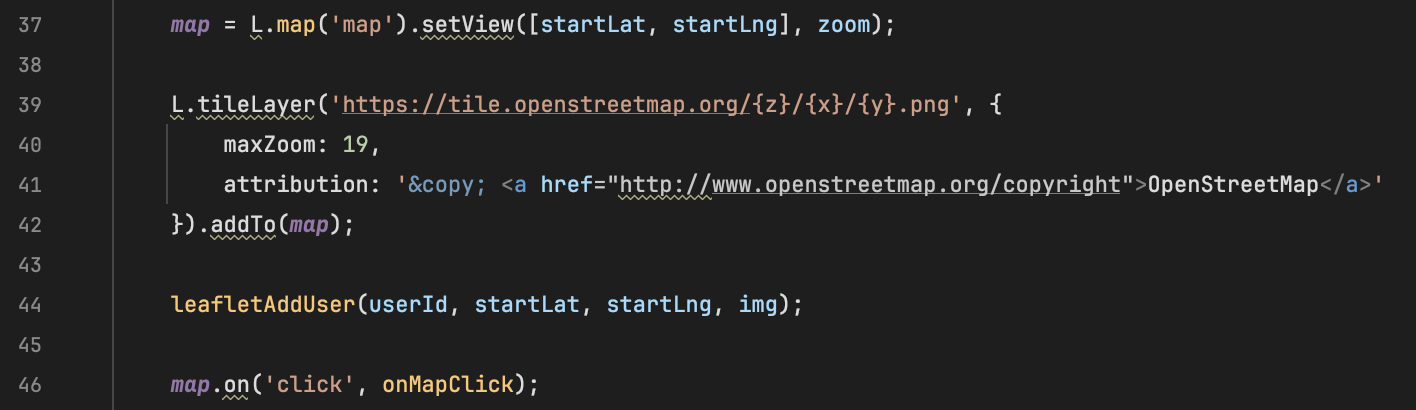
\includegraphics[width=14cm]{Assets/initLeaflet.png}
    \caption{Inițializarea hărții după ce componenta s-a randat.}
    \label{fig:initLeaflet}
\end{figure}

Orice iconiță adăugată pe hartă sunt un \textit{marker} cu o imagine ca și înfățișare. Pentru a pune un \textit{pin} spre exemplu, există o metodă numită \textit{SetPinLocationAsync} ce adaugă un \textit{marker} pe hartă cu \textit{asset-ul de pin}.
Toate asset-urile se află în \textit{wwwwroot/icons}: /textit{pin}, /textit{human}, /textit{driver} și /textit{currentCar} (ce indică că atât clientul cât și șoferul se află în mașină).
Metodele \textit{DrawRoute} și \textit{AddUser/Driver} ajută la trasarea traseului și adăugarea unui utilizator pe hartă.

\begin{figure}[H]
    \centering
    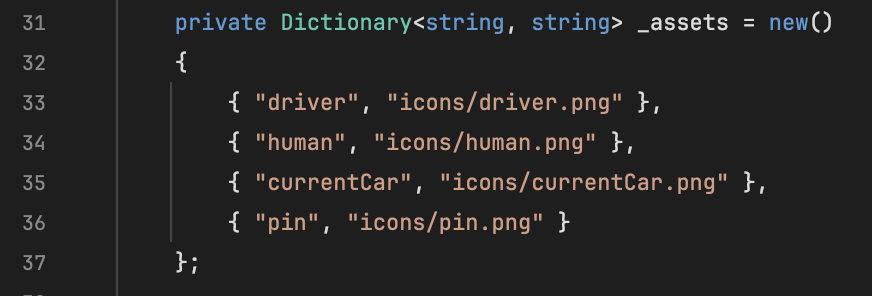
\includegraphics[width=14cm]{Assets/icons.png}
    \caption{Dicționarul ce face legătura dintre tipul de marker și imaginea de îl reprezintă.}
    \label{fig:icons}
\end{figure}

Același mecanism de afișare îl folosește și dialog-ul pentru a introduce cardul bancar. 
Se atașează input-urile de elementul \textit{div} cu ID-ul \textit{payment-element}. Acesta
validează un card bancar folosind API-ul Stripe, iar pentru a putea autoriza acest request,
se folosește de \textit{PublishKey} din dashboard-ul Stripe.

\begin{figure}[H]
    \centering
    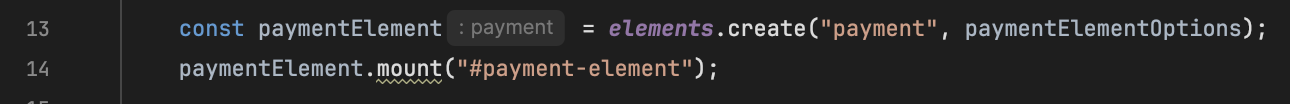
\includegraphics[width=14cm]{Assets/stripeMount.png}
    \caption{Atașarea input-ului pentru card bancar de elementul cu ID-ul \textit{payment-element}.}
    \label{fig:stripeMount}
\end{figure}

Toate tranzacțiile sunt se pot vedea în platfoma, dacă au fost cu succes, ce card a fost folosit sau de către ce customer.
Fiind în modul de testare, se poate folosi doar cardul cu numărul: \textit{4242 4242 4242 4242}, restul informațiilor
trebuind doar să fie corecte, nu să și existe.

\begin{figure}[H]
    \centering
    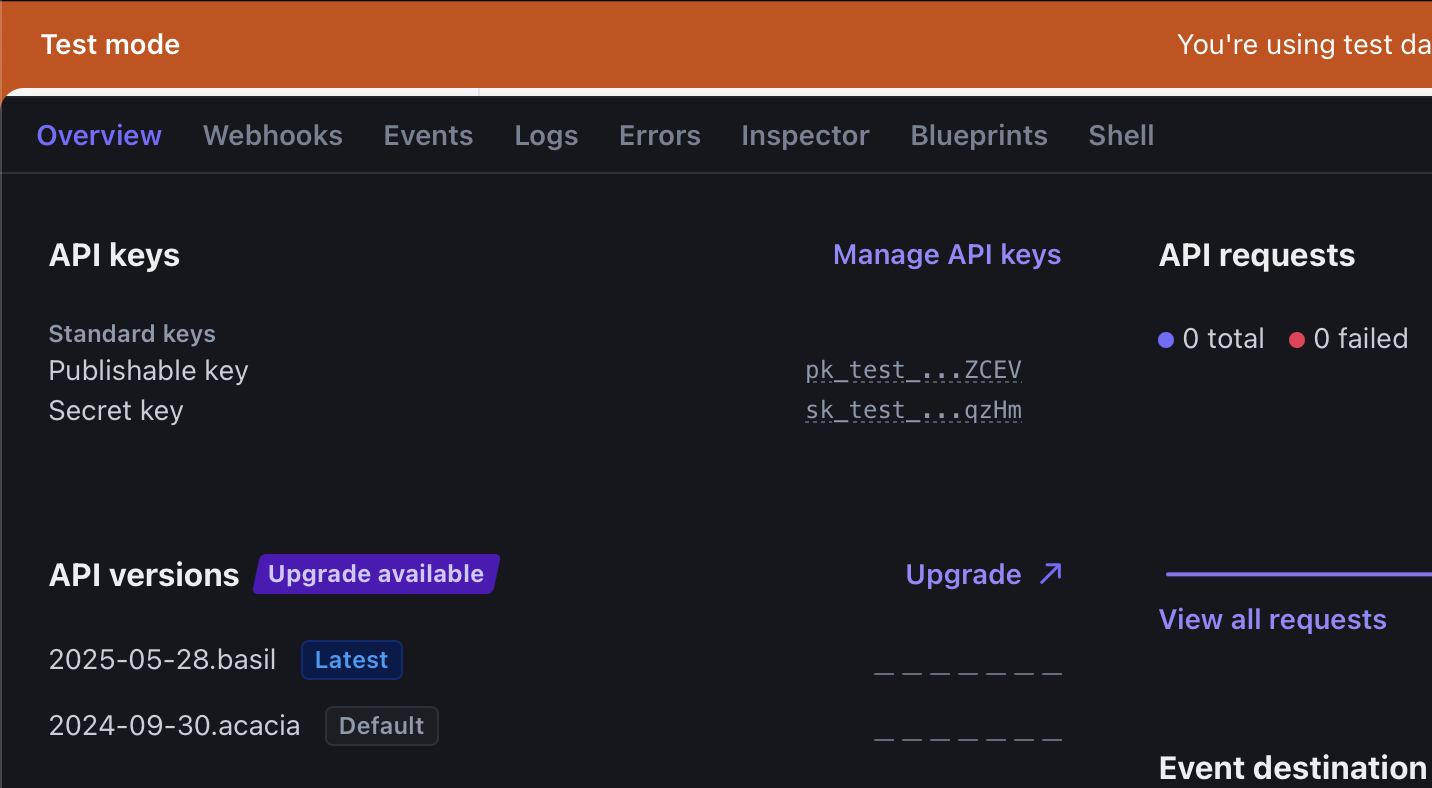
\includegraphics[width=14cm]{Assets/stripeSite.png}
    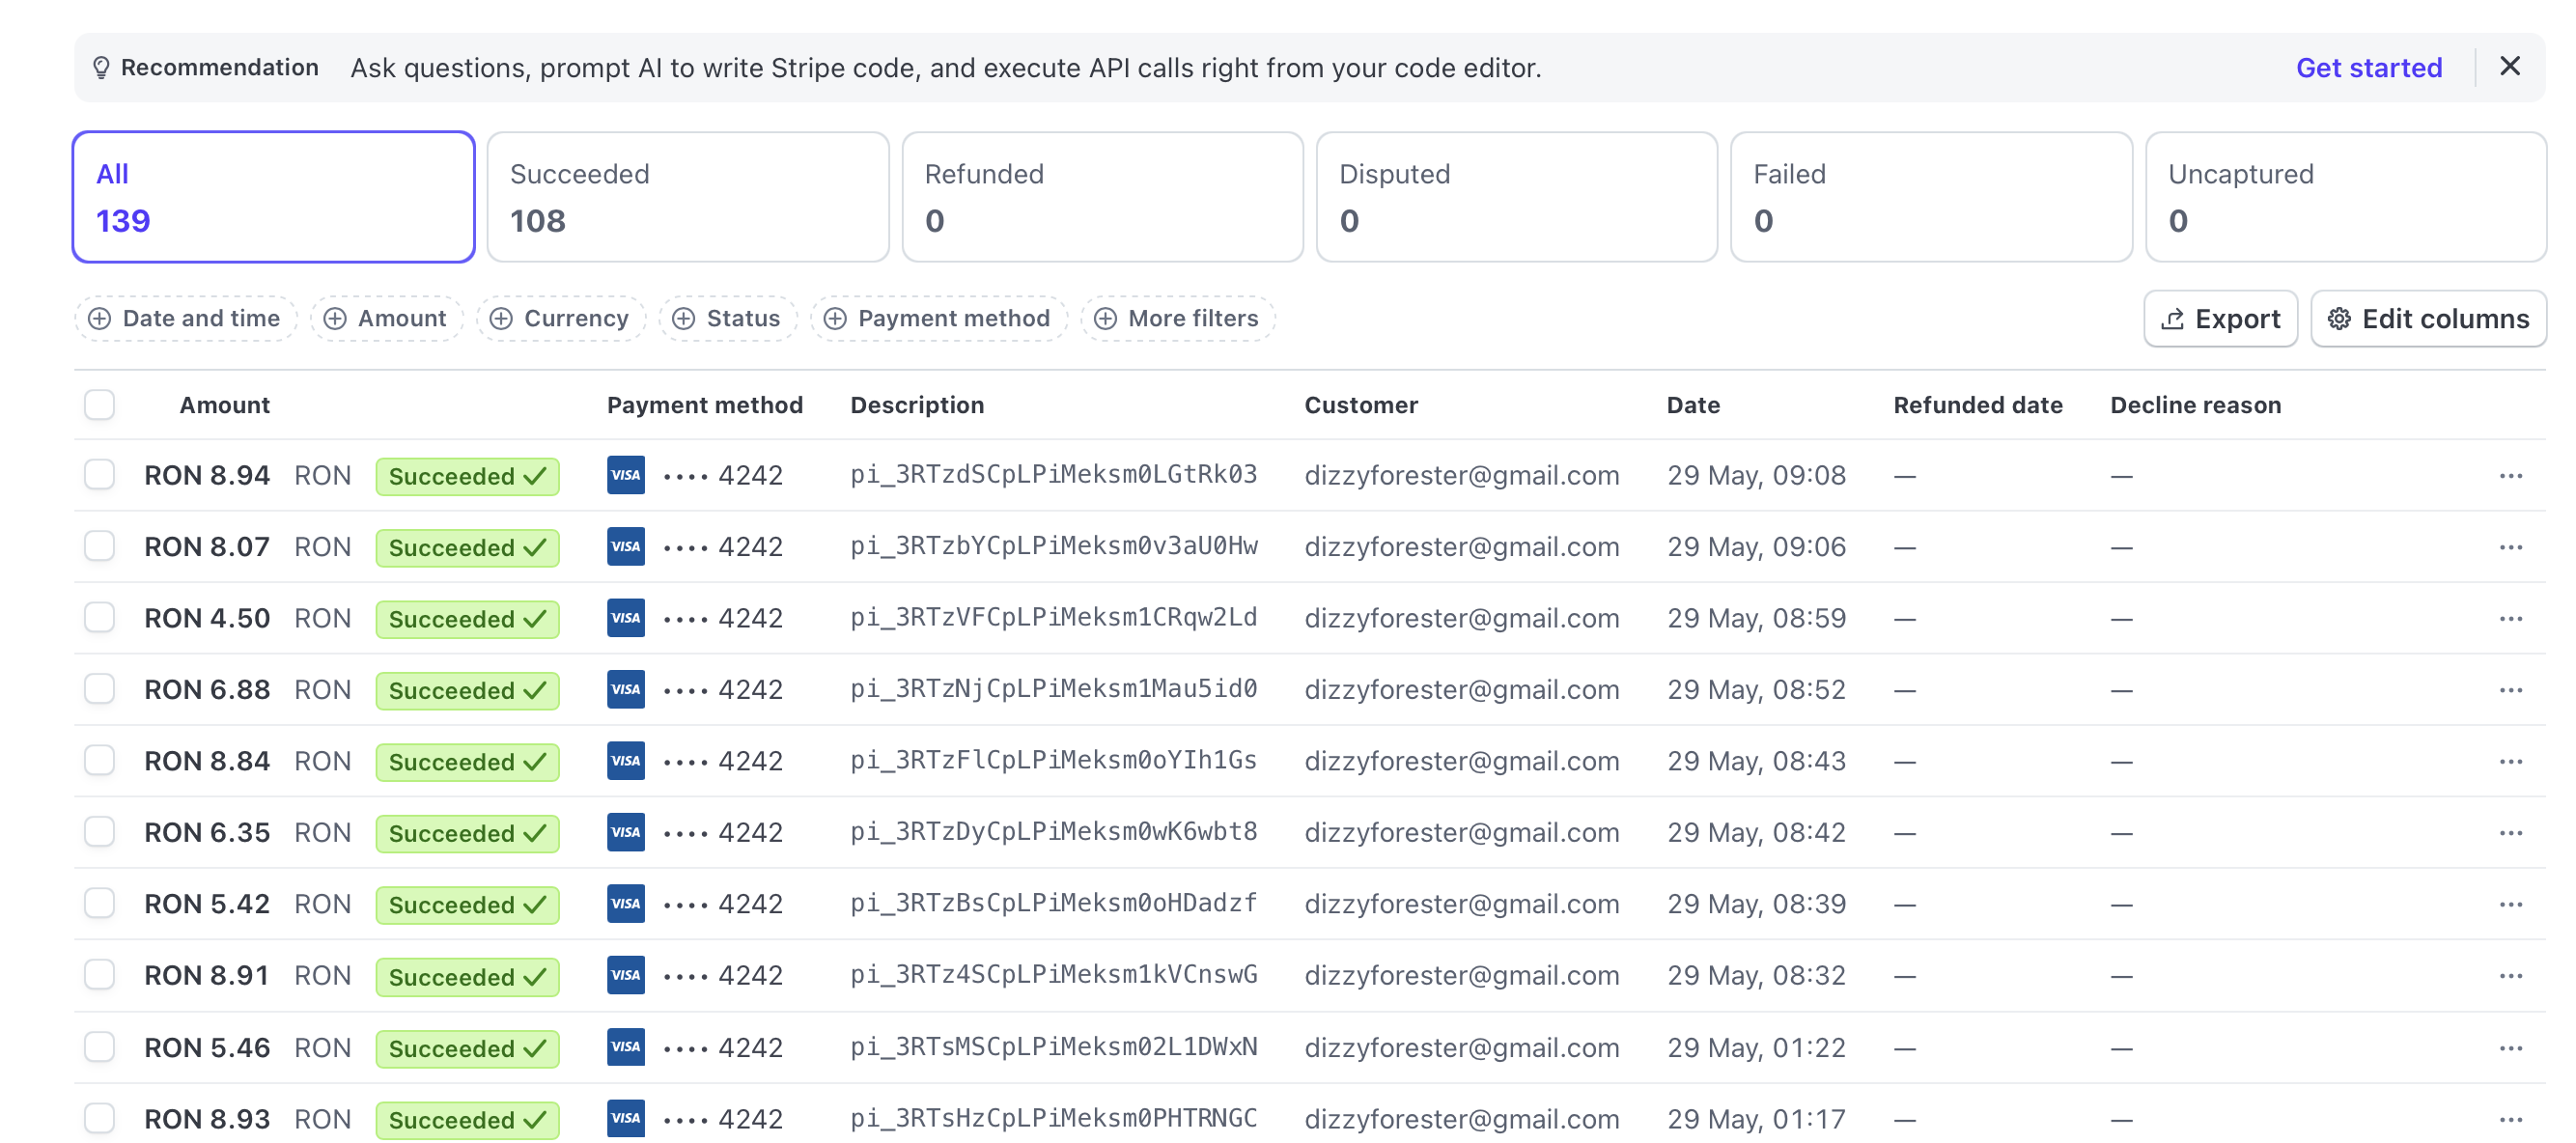
\includegraphics[width=14cm]{Assets/stripeHistory.png}
    \caption{Configurarea Stripe în dashboard-ul platformei și istoricul tranzacțiilor.}
    \label{fig:stripeSiteHistory}
\end{figure}

\section{Comunicarea între componente}
diagrama de cum comunica aplicatia
\subsection{Autentificare și autorizare}
\subsection{Pagina admin-ului}